\documentclass[12pt
,a4paper
,titlepage
,twoside
%,openany % ouvre les sections indifféremment sur la page de gauche ou de droite
]{book}

% Définition des marges de la page
\usepackage[left=3cm,right=3cm,top=2cm,bottom=2cm]{geometry}

% Paramétrages de la langue et de l'encodage
\usepackage[utf8x]{inputenc}
\usepackage[square,sort,comma,numbers]{natbib}
\usepackage[french]{babel}
\usepackage[T1]{fontenc}

%\usepackage{fontspec}
%\setmainfont{Linotype-AvenirNextLTPro.ttf}[
%BoldFont = Linotype-AvenirNextLTProBold.ttf,
%ItalicFont = Linotype-AvenirNextLTProItalic.ttf,
%BoldItalicFont = fLinotype-AvenirNextLTProBoldItalic.ttf
%]

% formules mathématiques
\usepackage{amsmath}
\usepackage{amsfonts}
\usepackage{amssymb}

% gestion des graphiques
\usepackage{graphicx}
\usepackage{transparent}

% Gestion des couleurs
\usepackage[usenames,dvipsnames]{xcolor}
\definecolor{inrae}{RGB}{0,163,166} % inrae
\definecolor{inraeclair}{RGB}{102,193,191}   % inrae clair
\definecolor{inraemedium}{RGB}{0,140,142}   % inrae medium
\definecolor{inraefonce}{RGB}{39,86, 98} % inrae foncé
\definecolor{vert}{RGB}{157,197,68} % vert
\definecolor{bleuclair}{RGB}{158,214,227} % bleu clair
\definecolor{bleufonce}{RGB}{66,48,137} % bleu foncé
\definecolor{gris}{RGB}{121,120,112}   % gris
\definecolor{argent}{RGB}{196,192,179} % argent
\definecolor{rouge}{RGB}{142,2,0} % rouge

% Redefinition des liens web
\usepackage{url}
\usepackage{hyperref}
\hypersetup{
urlcolor=inraefonce
,linkcolor=.
,colorlinks=true}


% Polices de caractères
\usepackage{times}
\usepackage{mathptmx} % times, y compris dans les formules mathématiques
\renewcommand{\familydefault}{\sfdefault}

% Insertion de code source dans le texte, à utiliser avec \begin{lstlisting} et \lstset{java|html|php...}
\usepackage{listings}
\lstset{
basicstyle=\footnotesize,        % the size of the fonts that are used for the code
  breakatwhitespace=false,         % sets if automatic breaks should only happen at whitespace
  breaklines=true,
  keepspaces=true,
}

% Définition des entêtes
\usepackage{fancyhdr}
\pagestyle{fancy}

% Redéfinition des titres de section
\usepackage{titlesec}

% Insertion de graphiques à des emplacements définis
\usepackage[abs]{overpic}

% règles typographiques de l'Imprimerie nationale
\usepackage[all]{nowidow}
\usepackage[
% frenchchapters renomme le premier chapitre, mais :
%	- cela pose problème dans la table des matières
%	- cela ne peut être utilisé qu'avec la renumérotation des chapitres activée
%frenchchapters,
parindent,
lastparline,
hyphenation
]{impnattypo}

% Renumérotation des chapitres
%\renewcommand{\thesection}{\Alph{section})}
%\renewcommand{\thesubsection}{\arabic{subsection} -}
%\renewcommand{\thesubsubsection}{\alph{subsubsection} -}
%\usepackage{engrec}
%\renewcommand{\theparagraph}{\engrec{paragraph})}
%\setcounter{secnumdepth}{4}

% Génération du code Ipsum lorem
\usepackage{blindtext}


% Definition des chapitres
%\usepackage{sectsty}
\titleformat{\chapter}[display]
{\normalfont\Huge\filcenter\sffamily\color{inrae}}
{\Large{\chaptertitlename~\thechapter}}
 {1em}{}

%{\titlerule
%% \vspace{1pc}%


\titleformat{\section}
{\color{inrae}\normalfont\Large\bfseries\sffamily}
{\color{inrae}\thesection}{1em}{}

\titleformat{\subsection}
{\color{inraefonce}\bfseries\sffamily}
{\color{inraefonce}\thesubsection}{1em}{}

\titleformat{\subsubsection}
{\color{gris}\bfseries\sffamily}
{\color{gris}\thesubsubsection}{1em}{}

% Bibliographie
% natbib est indispensable si la biblio contient des accents
% Options pour natbib (extrait de http://merkel.zoneo.net/Latex/natbib.php)
%    round: (par défaut) pour des parenthèses arondies (());
%    square: pour des crochets ([]);
%    curly: pour des accolades ({});
%    angle: pour des équerres (<>) ;
%    colon: (par défaut) pour séparer les citations multiples par deux points (:);
%    comma: pour utiliser une virgule comme séparateur;
%    authoryear: (par défaut) pour des citations auteurs-année;
%    numbers: pour des citations numériques;
%    super: pour des citations numériques en exposant, comme dans Nature;
%    sort: ordonne les citations multiples dans l'ordre dans lequel elles apparaissent dans la bibliographie;
%    sort&compress: comme sort mais en plus les citations numériques multiples sont comprimées, si possible (3-6, 15, par exemple);
%    longnamesfirst: transforme la première citation à une référence en une version étoilée (avec la liste complète des auteurs) et le citations suivantes normales (liste abbrégée);
%    sectionbib: pour redéfinir \thebibliography pour avoir une \section* à la place d'un \chapter*; valide seulement pour les classes de document possédant la commande \chapter; à utiliser avec le paquetage  chapterbib;
%    nonamebreak: garde tous les noms d'auteurs d'une citation sur une même ligne; celà cause des problèmes de débordement, mais permet de résoudre certains problèmes liés à hyperref.

% En cas de souci, supprimez les fichiers .aux et .bbi après modification des paramètres
% styles natbib natifs : abbrvnat, plainnat, unsrtnat
\bibliographystyle{unsrtnat}
\usepackage{hypernat}
% Ajout de la référence à la bibliographie dans la table des matières
\usepackage[nottoc, notlof, notlot]{tocbibind}

%Données de titre et d'auteur pour la page de garde
\newcommand{\titre}{Logiciel Collec-Science}
\newcommand{\sousTitre}{Installation, configuration et administration}
\newcommand{\auteur}{Éric Quinton}
\newcommand{\dateVersion}{1\ier{} mars 2020}
\newcommand{\version}{Version 2.4.0}
\usepackage[final]{pdfpages} 

\usepackage{lscape}
\usepackage{longtable}
\usepackage{float}
\usepackage{array}
\begin{document}
%Supprime les veuves et orphelines
\widowpenalty=10000
\clubpenalty=10000
\raggedbottom 

% Integrer la page de garde

\thispagestyle{empty}
\newgeometry{left=2cm,bottom=0.1cm}
\vspace*{4cm}
\textcolor{inrae}{\sffamily\Huge\bfseries\titre}\par
\textcolor{inrae}{\sffamily\Large\bfseries\sousTitre}\par
\textcolor{inrae}{\sffamily\dateVersion{} -- \version}\par

% Sigle INRAE
\vspace*{3cm}

\includegraphics{inrae}\par\bigskip
\textcolor{inrae}{\sffamily\Large Institut national de recherche pour}\par
\textcolor{inrae}{\sffamily\Large\bfseries l'agriculture, l'alimentation et l'environnement}\par\bigskip

% Logo INRAE

\vspace*{2cm}
\hspace{-5cm}
{\transparent{0.4}
\includegraphics[width=10cm]{sigle-inrae-plein}}

\vspace*{2cm}
   \textcolor{inrae}{\sffamily
   Site web de Collec-Science :
   {\large \href{https://www.collec-science.org}{https://www.collec-science.org} }
   }\par
\vspace*{1cm}
\textcolor{inrae}{\sffamily\auteur}\par

\textcolor{inrae}{\sffamily
Document distribué sous licence CC-BY}\par
  
\includegraphics[width=1cm]{cc-by} \href{https://creativecommons.org/licenses/by/4.0/fr/legalcode}{https://creativecommons.org/licenses/by/4.0/fr/legalcode}
\restoregeometry
% Définition des entêtes
\fancyhead{}
\fancyhead[CO]{\leftmark\sffamily}
\fancyhead[CE]{ \sffamily\titre{}}
\fancyfoot[CO]{\sffamily\thepage}
\fancyfoot[CE]{\sffamily\thepage}
% Redéfinition de \cleardoublepage pour créer une page totalement vide
\makeatletter
\def\cleardoublepage{\clearpage\if@twoside \ifodd\c@page\else
  \hbox{}
  \vspace*{\fill}

  \vspace{\fill}
  \thispagestyle{empty}
  \newpage
  \if@twocolumn\hbox{}\newpage\fi\fi\fi}
\makeatother

% \cleardoublepage permet de générer une page vide 
% si le chapitre ne commence pas sur la page de droite

% Ajout d'un préambule
\frontmatter
\cleardoublepage

% Table des matières
\tableofcontents


% Début réel du texte
\mainmatter
%\cleardoublepage

\chapter{Besoins nécessitant l'utilisation de services web}

\section{Définitions}

\begin{description}
\item[uid:] identifiant unique numérique au sein d'une base de données d'un échan\-tillon ;
\item[guid:] identifiant de type UUID\footnote{Les codes de type GUID ou UUID sont générés à partir de fonctions aléatoires ou cryptographiques, et garantissent qu'ils sont uniques quelle que soit la base de données qui les ont générés. Ainsi, il n'est pas possible d'obtenir deux codes identiques pour deux échantillons différents, ce qui permet de les identifier de manière sûre, comme pourrait le faire l'ADN pour des êtres humains.}, qui garantit de manière certaine l'identification d'un échantillon ;
\item [identifier :] identifiant \og métier \fg{} d'un échantillon;
\item [données \og métier \fg{} :] données permettant de caractériser un échantillon selon les critères nécessaires à son exploitation : contexte spécifique d'acquisition, taxon, données physico-chimiques ou biologiques, etc.
\item [instance, serveur, base de données, application :] implémentation d'une solution de gestion d'échantillons capable soit de fournir des services web, soit d'interroger des services web pour récupérer des informations.
\end{description}
\section{Présentation}
Collec est un logiciel de gestion de collections d'échantillons, dont l'objectif principal consiste à permettre de retrouver rapidement un échantillon stocké ou de récupérer les informations générales le concernant.

Écrit en PHP, les données sont stockées dans une base de données PostgreSQL. Le code de l'application est disponible à l'adresse \url{https://gitlab.com/Irstea/collec}. Il est disponible sous licence AGPL.

Le logiciel est bâti sur un modèle MVC, tous les accès étant gérés par l'appel à des modules déclarés dans un fichier spécifique. Il ne gère pas initialement les URL conviviales (implémenté à partir de la version 1.1).

La gestion matérielle des échantillons de laboratoire (ou d'expérimentations scientifiques) est une fonctionnalité largement demandée, mais peu couverte jusqu'à présent par les logiciels disponibles, et particulièrement dans le domaine de l'\textit{Open Source}. Collec, dont la première version remonte à l'automne 2016, fait l'objet d'un réel intérêt de la part de la communauté scientifique, ses fonctionnalités et sa facilité d'utilisation le rendant attractif.

Toutefois, il n'est pas conçu comme un système global de gestion de données à la fois techniques -- stockage des échantillons -- et de résultats d'analyse par exemple (pas d'informations métiers complexes\footnote{Dans la pratique, à partir de la version 1.1, il est possible de renseigner quelques informations métiers, mais de manière relativement frustre et sans permettre la complexité des actions envisageables avec des bases de données dédiées.}).
Il n'est pas non plus prévu de mettre en place un hébergement centralisé qui permettrait de gérer tous les échantillons de la sphère de recherche.

\textit{A contrario}, cette organisation permet de créer autant d'instances que néces\-saires, notamment pour gérer des saisies en mode décentralisé (bateau partant en campagne de sondage dans les mers du Sud, collecte d'échantillons depuis des zones non couvertes par Internet, par exemple).

Cette souplesse nécessite de prévoir des mécanismes soit d'interrogation de diverses instances, soit de récupération des informations concernant des échantillons provenant d'autres bases de données. 
Pour harmoniser les échanges ou les interrogations, la technologie des services web s'impose, en raison de la normalisation qu'elle apporte.

\subsection{Technique employée}

Les services web sont basés sur des requêtes HTTP, et échangent les données selon des formats définis. Dans la version actuelle des services web, seul le format Json est implémenté pour l'échange des informations.

\subsection{Forme des URL}
Les URL sont conçues, dans le cadre des services web, sous la forme d'URL conviviales, par exemple : \textit{http://collec/sw/v1/sample/4} pour récupérer l'échan\-tillon numéro 4.

\section{Définition des cas d'utilisation couverts par les services web}

SCHEMA

\subsection{Recherche d'échantillons}
La recherche d'échantillons doit pouvoir s'effectuer selon plusieurs critères :
\begin{itemize}
\item l'identifiant interne (\textit{uid});
\item l'identifiant principal ou des identifiants secondaires;
\item une fourchette de dates de création des échantillons;
\item un type d'échantillons;
\item un projet ou sous-collection;
\item une fourchette d'identifiants internes;
\item un code unique de type GUID ou UUID.
\end{itemize}

Elle retourne une liste d'échantillons correspondant aux critères indiqués. Le détail des informations retournées est spécifié dans la section \ref{sampleSearch}.

Pour permettre cette recherche, d'autres services sont nécessaires, notamment pour récupérer la liste des types d'échantillons ou la liste des projets (ou sous-collections).

\subsection{Liste des projets ou sous-collections}
Ce service doit permettre de récupérer la liste des projets ou sous-collections autorisés pour un utilisateur, pour qu'ils puissent servir dans le cadre de la recherche.

\subsection{Liste des types d'échantillons}
Ce service récupère la liste exhaustive des types d'échantillons utilisés dans l'instance distante, pour une utilisation dans le cadre de la recherche.

\subsection{Liste des types d'identifiants secondaires}
Ce service récupère la liste exhaustive des types d'échantillons secondaires, pour une utilisation dans le cadre de la recherche des échantillons.

\subsection{Récupération des données d'un échantillon}
Ce service permet de récupérer l'ensemble des données concernant un échan\-tillon, y compris les données \og métiers \fg{} si l'utilisateur dispose des droits néces\-saires pour les consulter.

Les données récupérées sont suffisamment complètes pour être intégrées dans l'instance \textit{Collec} courante, par exemple pour éviter de les ressaisir suite au prêt d'un échantillon par un laboratoire.

Elles permettent également une visualisation détaillée de l'échantillon consi\-déré, et contiennent, le cas échéant\footnote{si l'utilisateur dispose des droits adéquats et si l'échantillon dispose de ces informations}, les données \og métiers \fg{} associées.

\subsection{Récupération des données d'une liste d'échantillons}

Il s'agit d'une variante du service web précédent. La liste des échantillons à récupérer est fournie dans une collection Json, soit en utilisant l'UID, soit en utilisant le GUID.

\section{Contraintes liées à la sécurité}

Les instances Collec sont prévues pour donner un accès en lecture à toutes les données des échantillons disponibles, dès lors que l'utilisateur s'est identifié. Cela permet ainsi de connaître, par exemple, le produit utilisé pour la conservation ou d'autres informations nécessaires pour la gestion quotidienne des collections.

Toutefois, les données \og métiers \fg ne sont accessibles qu'aux personnes habilitées à les consulter. Dans la pratique, dans Collec, les échantillons sont associés à un projet, et seuls les utilisateurs rattachés à celui-ci peuvent prendre connaissance de ces informations.
Cela impose une gestion particulière des accès lors de l'interrogation par l'intermédiaire des services web, qui sera décrite dans le chapitre \ref{habilitation}.

Le protocole d'identification des utilisateurs dans l'instance distante est basé sur le protocole Oauth v2.



\chapter{Installer le logiciel}

\section{Consultez la documentation du framework !}

Le logiciel a été conçu à partir du framework \textit{Prototypephp}. La documentation associée \cite{pphp-doc} récapitule l'ensemble des informations nécessaires pour réaliser l'installation générale (configuration du serveur, définition des droits d'accès, etc.).

De nombreuses passages ont été repris ici, mais il n'est pas inutile de se référer au document d'origine. 

\section{Configuration du serveur}
La configuration est donnée pour un serveur Linux fonctionnant avec Ubuntu 16.04 LTS Server. Elle peut bien sûr être adaptée à d'autres distributions Linux. Par contre, rien n'a été prévu pour faire fonctionner l'application directement dans une plate-forme windows, même si, en théorie, cela devrait être possible.

\subsection{Configuration d'Apache}
Les modules suivants doivent être activés :
\begin{lstlisting}
a2enmod ssl
a2enmod headers
a2enmod rewrite
\end{lstlisting}

\subsection{Modules PHP nécessaires}
Modules complémentaires nécessaires :
\begin{itemize}
\item \textit{php-mbstring}
\item \textit{php-pgsql}
\item \textit{php-xdebug} pour les phases de mise au point
\item \textit{php-curl} (ou \textit{php5-curl} pour PHP5) pour l'identification via un serveur CAS.
\end{itemize}
La génération des étiquettes nécessite les paquetages suivants :
\begin{itemize}
\item \textit{php-gd} (ou \textit{php5-gd} pour PHP5)
\item \textit{fop} (qui inclut des bibliothèques java)
\end{itemize}

Le stockage et l'affichage des photos nécessite :
\begin{itemize}
\item \textit{php-imagick} (ou \textit{php5-imagick} pour PHP5)
\end{itemize}

\subsection{Configuration de l'hôte virtuel et de SSL}
L'application ne fonctionne qu'en mode SSL, les cookies de session n'étant pas transmis sur des liens non chiffrés. Voici un exemple de configuration à insérer dans le fichier \textit{/etc/apache2/sites-available/default-ssl}
\begin{lstlisting}
    <Directory /var/www/html>
        Options FollowSymLinks MultiViews
        AllowOverride all
        Order allow,deny
        allow from all
    </Directory>

    SSLProtocol All -SSLv2 -SSLv3
    SSLHonorCipherOrder On
    SSLCipherSuite ECDHE-RSA-AES128-SHA256:AES128-GCM-SHA256:HIGH:
    !MD5:!aNULL:!EDH:!RC4
    SSLCompression off
\end{lstlisting}

La chaîne \textit{SSLCipherSuite} est donnée à titre d'exemple, d'autres configurations plus modernes peuvent être implémentées (\textit{cf.} \cite{tls}).

Pour activer le mode SSL dans Apache :
\begin{lstlisting}
chmod -R g+r /etc/ssl/private
usermod www-data -a -G ssl-cert
a2ensite default-ssl
service apache2 restart
\end{lstlisting}


\subsection{Configuration du dossier d'installation}

\subsubsection{Mécanisme pour faire cohabiter plusieurs instances avec le même code}
\label{dnsmultiple}
Il est possible d'utiliser le même code applicatif pour alimenter des bases de données différentes (ou des données stockées dans des schémas différents). Cette fonctionnalité est basée sur l'attribution d'entrées DNS différentes. 

Le mécanisme est décrit dans le schéma \ref{dnsmultipleschema}, page \pageref{dnsmultipleschema}.

\begin{figure}[H]
\label{dnsmultipleschema}
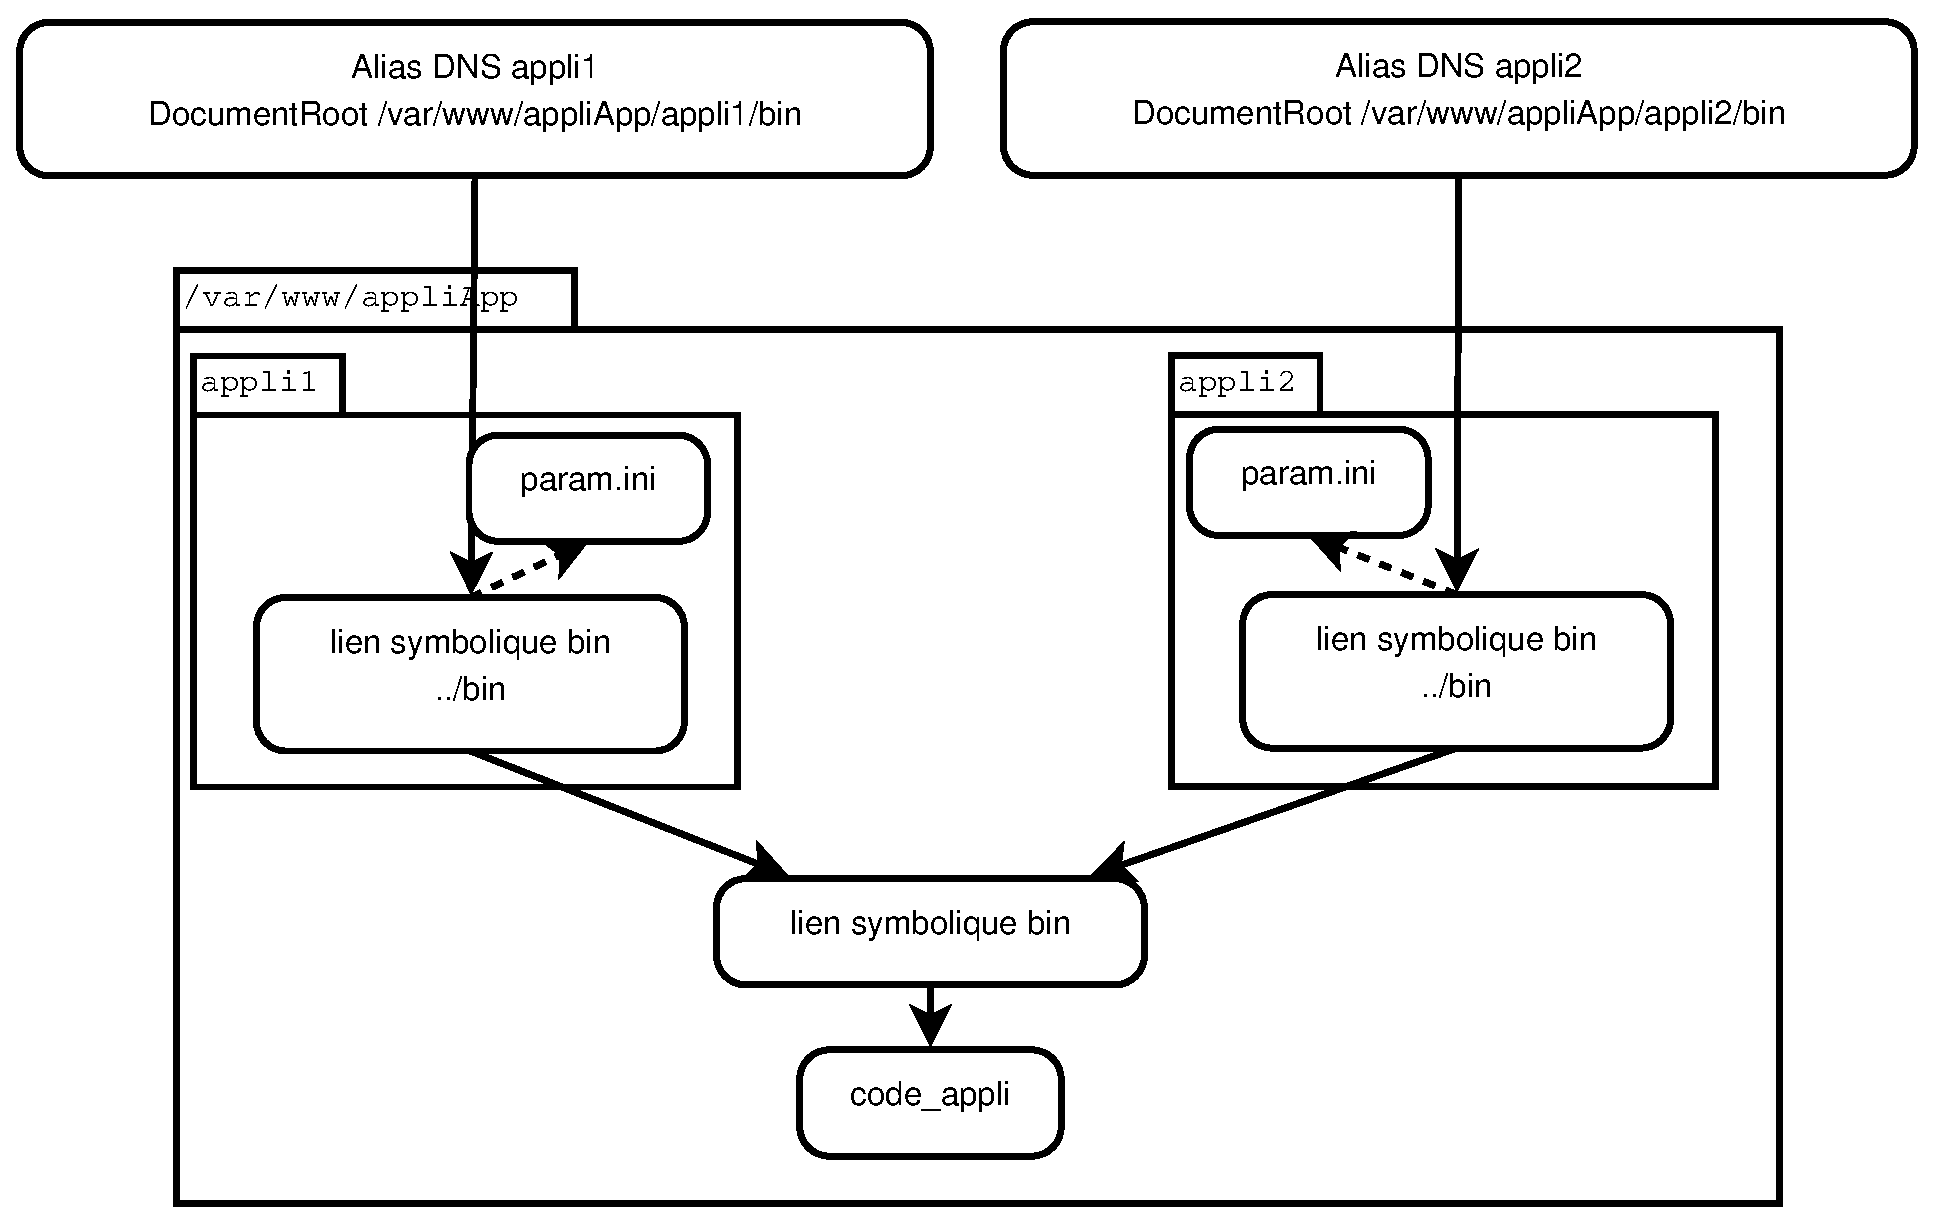
\includegraphics[width=\linewidth]{images/dnsmultiple}
\caption{Schéma général d’implémentation pour utiliser le même code avec des noms d’application et des jeux de données différents}
\end{figure}

Dans le paramétrage de l’alias DNS (en principe, dans \textit{/etc/apache2/sites-available}), l’application pointe vers le dossier \textit{/var/www/appliApp/appli1/bin}. \textit{/var/www} correspond à la racine du site web, \textit{appliApp} au dossier racine de l’application, \textit{appli1} au dossier spécifique de l’alias DNS. Ce dossier \textit{appli1} ne contient que deux fichiers : \textit{param.ini}, qui contient les paramètres spécifiques, et \textit{bin}, qui est un lien symbolique vers le dossier \textit{../bin}.

Le dossier \textit{../bin} (donc, dans\textit{ /var/www/appliApp}) est lui aussi un alias qui pointe vers le code réel de l’application, ici \textit{code\_appli}. Le fichier \textit{param.inc.php} décrit l’entrée suivante : 
\begin{lstlisting}
$paramIniFile = "../param.ini"; 
\end{lstlisting}

Le fichier \textit{param.ini} sera cherché dans le dossier parent du code de l’application, c’est à dire soit dans \textit{appli1}, soit dans \textit{appli2} dans cet exemple. Il suffit qu’il contienne les paramètres adéquats pour rendre l’application utilisable dans des contextes différents à partir du même code initial.



Le fichier \textit{param.ini} est le dernier qui est traité par l'application pour récupérer les paramètres. Ceux-ci sont lus dans l'ordre suivant :

\textbf{param/param.default.inc.php $\rightarrow$ param/param.inc.php $\rightarrow$ ../param.ini}

\textit{param.ini} contiendra les entrées spécifiques liées au DNS utilisé pour accéder à l'application, en principe tout ou partie de celles-ci :
\begin{lstlisting}
APPLI_titre=Gestion des collections EABX
BDD_schema=col, public, gacl
BDD_login=compte_de_connexion
BDD_passwd=mot_de_passe_de_connexion
BDD_dsn=pgsql:host=serveur;dbname=base_de_donnees;sslmode=require
GACL_aco=col
APPLI_code=proto
\end{lstlisting}



\subsubsection{Droits à attribuer au serveur web}

Le serveur web doit pouvoir accéder en lecture à l'ensemble des fichiers de l'application, et en écriture à deux dossiers :
\begin{itemize}
\item \textit{display/templates\_c} : fichier utilisé par Smarty pour compiler les modèles de documents HTML ;
\item \textit{temp} : dossier de génération des images et des fichiers temporaires.
\end{itemize}

Voici un exemple de script utilisé pour positionner les droits :

\begin{lstlisting}
#!/bin/bash
cp ../param/* param/
chmod -R 770 .
setfacl -R -m u:www-data:rx .
setfacl -R -m d:u:www-data:rx .
mkdir display/templates_c
setfacl -R -m u:www-data:rwx display/templates_c
setfacl -R -m d:u:www-data:rwx display/templates_c
setfacl -R -m u:www-data:rwx temp
setfacl -R -m d:u:www-data:rwx temp
setfacl -R -m d:o::- .
rm -Rf database
rm -Rf test
rm -f param.ini
\end{lstlisting}

Dans cet exemple, le dossier \textit{../param} contient le fichier \textit{param.inc.php}, qui dispose des paramètres spécifiques à l'implémentation.

Le script est à lancer à la racine du dossier contenant l'application.

\section{Configurer l'application}

L'application est configurable par l'intermédiaire de trois fichiers, comme nous venons de le voir :

\textbf{param/param.default.inc.php $\rightarrow$ param/param.inc.php $\rightarrow$ ../param.ini}

Le premier fichier contient les paramètres par défaut. Il est systématiquement fourni à chaque nouvelle version de l'application.

Le second est spécifique de l'implémentation. Il comprend notamment les informations liées à la connexion à la base de données, à la méthode d'identification, ou à la recherche des attributs dans l'annuaire LDAP. 

le troisième est destiné à offrir la possibilité d'accéder, à partir du même code applicatif, à plusieurs bases de données différentes (\textit{cf.} \ref{dnsmultiple} \textit{\nameref{dnsmultiple}}).

Voici les principaux paramètres utilisés :

\subsection{Connexion à la base de données}

Dans la pratique, deux connexions sont nécessaires : l'une pour accéder à la base des droits, l'autre aux données proprement dites. Voici les paramètres à définir :

\begin{longtable}{|p{5cm}|p{10cm}|}
\hline
\textbf{Variable} & \textbf{Signification} \\
\hline
\endhead
BDD\_login & compte de connexion à la base de données \\
\hline
BDD\_passwd & mot de passe associé\\
\hline
BDD\_dsn & adresse de la base de données sous forme normalisée\\
\hline
BDD\_schema & schéma utilisé (plusieurs schémas peuvent être décrits, en les séparant par une virgule - fonctionnement propre à Postgresql)\\
\hline
GACL\_dblogin & compte de connexion à la base de données des droits\\
\hline
GACL\_dbpasswd & mot de passe associé\\
\hline
GACL\_dsn & adresse normalisée \\
\hline
GACL\_schema & schéma utilisé\\
\hline
GACL\_aco & nom du code de l'application utilisé dans la gestion des droits\\
\hline
\caption{Variables utilisées pour paramétrer les connexions}
\end{longtable}

\subsection{Identification des utilisateurs}

\begin{longtable}{|p{5cm}|p{10cm}|}
\hline
\textbf{Variable} & \textbf{Signification} \\
\hline
\endhead
ident\_type & Type d'identification supporté. L'application peut gérer \textbf{BDD} (uniquement en base de données),\textbf{LDAP} (uniquement à partir d'un annuaire LDAP) \textbf{LDAP-BDD} (d'abord identification en annuaire LDAP, puis en base de données), et \textbf{CAS} (serveur d'identification \textit{Common Access Service}\footnote{serveur externe gérant l'identification des utilisateurs, et renvoyant à l'application le login utilisé})\\
\hline
CAS\_plugin & Nom du plugin utilisé pour une connexion CAS \\
\hline
CAS\_address & Adresse du serveur CAS\\
\hline
CAS\_port & Systématiquement 443 (connexion chiffrée)\\
\hline
LDAP & tableau contenant tous les paramètres nécessaires pour une identification LDAP \\
\hline
privateKey & clé privée utilisée pour générer les jetons d'identification \\
\hline
pubKey & clé publique utilisée pour générer les jetons d'identification \\
\hline
tokenIdentityValidity & durée de validité, en secondes, des jetons d'identification\\
\hline
\caption{Variables utilisées pour paramétrer l'identification}
\end{longtable}

L'application permet de conserver l'identification plus longtemps que celle définie dans le serveur, en rejouant la connexion avec un jeton d'identification chiffré. Cela évite, par exemple, de devoir se ré-identifier toutes les heures si on accède au logiciel à partir d'un terminal mobile (smartphone ou tablette, par exemple).

Les trois dernières variables permettent de configurer ce mode d'identification. Pour plus d'informations, consultez \cite{token}.

\subsection{Configuration de l'accès à l'annuaire LDAP}

Les paramètres LDAP sont stockés dans un tableau :
\begin{lstlisting}
$LDAP = array(
		"address"=>"localhost",
		"port" => 389,
		"rdn" => "cn=manager,dc=example,dc=com",
		"basedn" => "ou=people,ou=example,o=societe,c=fr",
		"user_attrib" => "uid",
		"v3" => true,
		"tls" => false,
		"groupSupport"=>true,
		"groupAttrib"=>"supannentiteaffectation",
		"commonNameAttrib"=>"displayname",
		"mailAttrib"=>"mail",
		'attributgroupname' => "cn",
		'attributloginname' => "memberuid",
		'basedngroup' => 'ou=example,o=societe,c=fr'
);
\end{lstlisting}


L'application peut non seulement identifier les utilisateurs auprès de l'annuaire LDAP, mais également récupérer les groupes auxquels ils appartiennent dans celui-ci.

Voici les paramètres à indiquer dans ce cas de figure : 
\begin{longtable}{|p{5cm}|p{10cm}|}
\hline
\textbf{Variable} & \textbf{Signification} \\
\hline
\endhead
address &  adresse de l'annuaire\\
\hline
port & 389 en mode non chiffré, 636 en mode chiffré\\
\hline
rdn & compte de connexion, si nécessaire \\
\hline
basedn & base de recherche des utilisateurs\\
\hline
user\_attrib & nom du champ contenant le login à tester\\
\hline
v3 & toujours à \textit{true}\\
\hline
tls & \textit{true} en mode chiffré\\
\hline
groupSupport & \textbf{true} si l'application recherche les groupes d'appartenance du login dans l'annuaire\\
\hline
groupAttrib & Nom de l'attribut contenant la liste des groupes d'appartenance\\
\hline
commonNameAttrib & Nom de l'attribut contenant le nom de l'utilisateur\\
\hline
mailAttrib & Nom de l'attribut contenant l'adresse mail de l'utilisateur\\
\hline
attributgroupname & Attribut contenant le nom du groupe lors de la recherche des groupes (cn par défaut)\\
\hline
attributloginname & attribut contenant les membres d'un groupe\\
\hline
basedngroup & base de recherche des groupes \\
\hline
\caption{Variables utilisées pour paramétrer l'accès à l'annuaire LDAP}
\end{longtable}

\subsection{Paramètres spécifiques}
\label{paramspec}

\begin{longtable}{|p{5cm}|p{10cm}|}
\hline
\textbf{Variable} & \textbf{Signification} \\
\hline
\endhead
GACL\_aco & nom du code de l'application utilisé dans la gestion des droits (\textit{cf.} \ref{droits} \textit{\nameref{droits}}, page \pageref{droits} )\\
\hline
APPLI\_code & Code interne de l'application. \textbf{Ce code est essentiel} : il sera inscrit dans les codes-barres générés, pour s'assurer qu'un échantillon est bien issu de la base de données concernée\\
\hline
\caption{Variables spécifiques}
\end{longtable}

\section{Créer la base de données}

La base de données est composée de deux schémas : l'un pour stocker les informations d'identification, les droits d'accès et les traces, l'autre pour les données proprement dites.

Le schéma \textit{public} ne devrait jamais être utilisé pour stocker l'information : réservez-le pour les composants communs, comme Postgis si c'est nécessaire.

Les tables de gestion des droits peuvent être communes à plusieurs jeux / applications différentes : la variable \textit{GACL\_aco} permet de séparer la gestion des droits pour chaque application, tout en travaillant à partir des mêmes utilisateurs (répartis le cas échéant dans des groupes différents selon le jeu de données considéré).

Les scripts de création des schémas dans la base de données sont stockés dans le dossier \textit{install}. 



\subsection{Créer les tables de gestion des droits}
Script à utiliser : \textit{gacl\_create.sql}. Les tables nécessaires vont être créées dans le schéma \textit{gacl} (ne modifiez pas le nom du schéma).

Le script crée un compte d'administration par défaut :
\begin{itemize}
\item login : \textbf{admin}
\item mot de passe : \textbf{password}
\end{itemize}

Il devra être supprimé quand un autre compte d'administration aura été créé.

Lles droits par défaut sont positionnés pour le projet \textit{appli} (variable \textit{\$GACL\_aco} dans les fichiers de paramètres de l'application).


\subsection{Créer les tables applicatives}
Script à utiliser : \textit{col\_create.sql}.

Par défaut, le script crée un schéma appelé \textit{col}. Il est possible de créer plusieurs schémas différents, si l'application supporte plusieurs jeux de données (\textit{cf.} \ref{dnsmultiple} \textit{\nameref{dnsmultiple}}, page \pageref{dnsmultiple}). Dans ce cas de figure, remplacez \textit{col} par le nom du schéma voulu dans les deux premières lignes du script.

\subsection{Login de connexion}

Il est fortement conseillé de créer deux logins de connexion, un pour le schéma des droits, l'autre pour les schémas applicatifs. Ces logins ne doivent pouvoir être utilisés que depuis le serveur web hébergeant l'application.

Cette opération est possible en modifiant le fichier \textit{/etc/postgresql/9.5/main/pg\_hba.conf} selon ce principe :

\begin{lstlisting}
# Connexions pour les serveurs web 
host nom_database userGacl adresse_serveur/32 md5 
host nom_database userData adresse_serveur/32 md5
\end{lstlisting}

et en rechargeant ensuite la configuration de Postgresql avec la commande :
\begin{lstlisting}
service postgresql reload
\end{lstlisting}

\subsection{Droits sur les tables}

Le compte utilisé pour la connexion au schéma des droits doit pouvoir modifier les informations présentes dans l'ensemble des tables de \textit{gacl}. Il ne doit pas pouvoir accéder aux autres schémas (hormis \textit{public}).

Le compte utilisé pour accéder aux schémas des données doit pouvoir modifier l'ensemble des informations dans les schémas de données, et lire la table \textit{gacl.aclgroup}.

Le plus simple est d'utiliser le logiciel \textit{pgAdmin} \cite{pgadmin} pour attribuer les droits.

\subsection{Scripts de modification}

Lors de la livraison de nouvelles versions, il est possible que des scripts de modification soient livrés pour mettre à niveau la base de données. Ces scripts doivent être exécutés dans tous les schémas contenant des données applicatives.

\section{Mise en production}

Une fois l'application configurée, et après avoir créé un nouveau compte d'administration :
\begin{itemize}
\item supprimez le compte \textit{admin}, livré par défaut, qui ne doit pas être conservé. Sa désactivation n'est pas suffisante : si pour une raison ou pour une autre le compte est réactivé, n'importe qui pourra récupérer les droits totaux ;
\item supprimez le dossier \textit{install} qui contient les scripts de création des tables ;
\item déplacez le dossier \textit{database}, qui contient la documentation d'installation et de configuration (elle n'a pas à rester accessible depuis le site web) ;
\item faites une revue des droits, pour vous assurer que tout est correctement configuré.
\end{itemize}

Vous pouvez également tester si la configuration du serveur est correcte en recourant à ZAProxy \cite{zaproxy}, qui analysera la communication entre le serveur et un navigateur et identifiera les problèmes éventuels de non conformité (mauvaise réécriture des entêtes HTML suite à une mauvaise configuration du serveur Apache, par exemple).

\chapter{Administrer l'application}

\section{Gérer les droits}
\label{droits}

Depuis la version 1.1, les scripts de création des bases de données intègrent la génération initiale des groupes et des droits associés, ceci afin de faciliter la phase de mise en route.

Toutefois, vous devrez créer des groupes d'utilisateurs correspondant à vos projets, et modifier ensuite les projets pour donner les droits adéquats aux groupes créés (\textit{cf.} \ref{projet}, page \pageref{projet}).

\subsection{Principe général}

Les droits sont gérés selon le principe initialement utilisé dans la bibliothèque PHPGACL \cite{phpgacl}, aujourd'hui obsolète. 

Les logins sont déclarés dans des groupes organisés de manière hiérarchique : un groupe hérite des droits attribués à ses parents.

Les droits utilisés dans le logiciel sont associés à des groupes. Il est possible d'attribuer plusieurs droits à un même groupe, et un droit peut être détenu par des groupes différents.

Si le paramètre \textit{\$LDAP["groupSupport"]} est positionné à \textit{true}, les groupes dont fait partie le compte LDAP sont également récupérés. Si ces groupes se voient attribués des droits, les comptes associés les récupéreront automatiquement.

Voici le schéma des tables utilisées pour gérer les droits :

\begin{figure}[H]
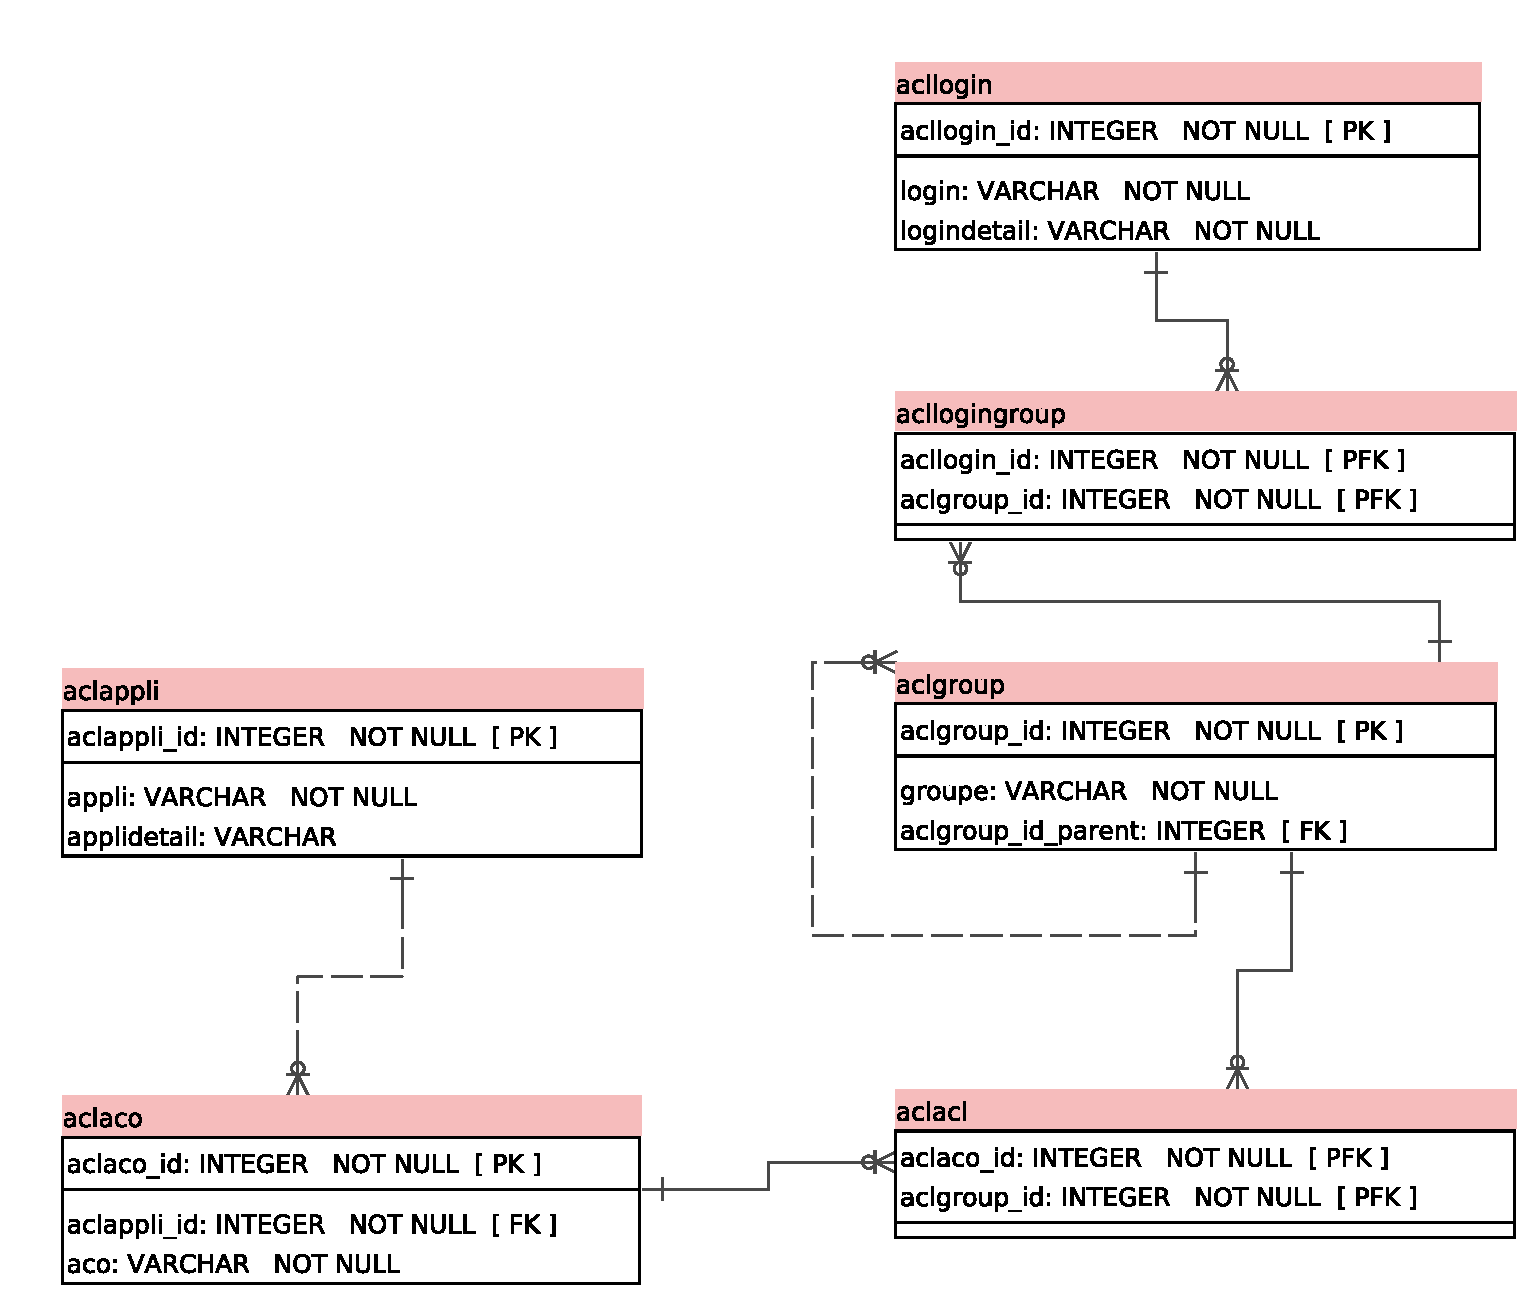
\includegraphics[width=\linewidth]{images/acl_only}
\caption{Schéma des tables utilisées pour gérer les droits}
\end{figure}

Voici la description des tables :
\begin{description}
\item[acllogin] : liste des logins utilisés. Si un compte est créé dans la base locale d'identification, un enregistrement est également créé dans cette table. Pour les identifications LDAP ou CAS, ils doivent être identiques. Si seuls les groupes LDAP sont utilisés pour un compte, il n'a pas besoin d'être décrit ici ;
\item[aclappli] : liste des applications gérées. Il est possible de gérer, à partir de la même base de données, plusieurs ensembles de droits, qui utilisent les mêmes logins.
\item[aclaco] : liste des droits déclarés dans l'application ;
\item[aclgroup] : liste des groupes contenant les logins, et qui détiennent les droits. Un groupe peut hériter d'un autre groupe. Les droits associés au groupe parent sont également attribués au groupe hérité ;
\item[acllogingroup] : table permettant de déclarer les logins associés à un groupe ;
\item[aclacl] : table décrivant les droits détenus par un groupe.
\end{description}

Le module d'administration permet de saisir toutes ces informations. Il faut que l'utilisateur dispose du droit \textit{admin}, c'est à dire qu'il fasse partie du groupe \textit{admin} (configuration par défaut à l'initialisation de la base des droits) pour pouvoir accéder à ces fonctions.

\subsection{Créer un nouvel utilisateur}

Les utilisateurs peuvent être issus soit de l'annuaire LDAP, soit de la base interne. 
Pour créer un nouvel utilisateur dans la base locale :
\begin{itemize}
\item \textit{Administration $\rightarrow$ Liste des comptes }
\item \textit{Nouveau login}
\item renseignez au minimum le login.
\end{itemize}

\begin{figure}[H]
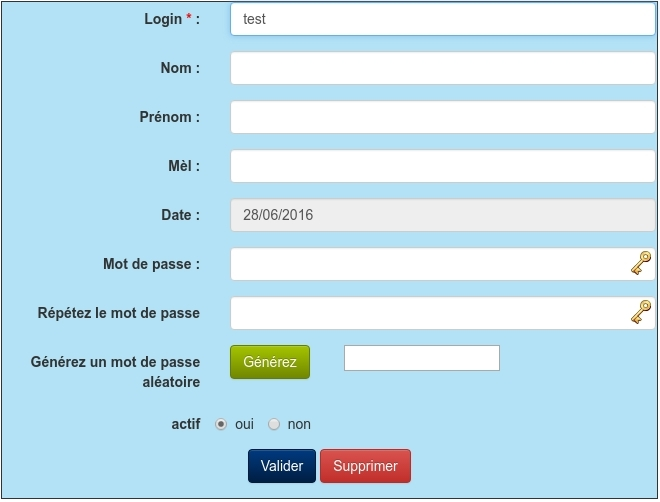
\includegraphics[width=\linewidth]{images/user_create}
\caption{Écran de saisie d'un login de connexion}
\end{figure}

Pour créer le mot de passe, vous pouvez cliquer sur le bouton \textit{Générez}, qui  en générera un automatiquement. Envoyez-le par mél à son destinataire (par \textit{copier-coller}), en lui demandant de le modifier à la première connexion (icône en forme de clé, dans le bandeau, en haut à droite).

Les mots de passe doivent respecter les règles suivantes :
\begin{itemize}
\item ils doivent avoir une longueur minimale de 8 caractères ;
\item ils doivent comprendre trois types de caractères différents parmi les minuscules, majuscules, chiffres et caractères de ponctuation ;
\item ils ne peuvent pas être réutilisés pour le même login ;
\item les mots de passe n'expirent pas.
\end{itemize}

Les mots de passe sont stockés sous forme d'empreinte, calculée en rajoutant un sel\footnote{chaîne de caractère rajoutée au mot de passe -- en général le login ou un identifiant -- qui permet d'éviter que deux mots de passe identiques, associés à deux logins différents, aient la même empreinte} et encodés en SHA256 : ils ne peuvent pas être retrouvés en cas de perte.

L'application n'intègre pas de module permettant de régénérer automatiquement un mot de passe en cas de perte : c'est au responsable applicatif d'en fournir un nouveau.

La création d'un compte entraîne la création d'une entrée identique dans la table des \textit{acllogin}, utilisée pour attribuer les droits.

Pour désactiver temporairement un compte, sélectionnez \textit{non} dans la zone \textit{actif}. Si le compte ne doit plus être utilisé, supprimez-le.

Attention : si le compte disposait des droits d'administration, assurez-vous que vous avez toujours un compte disposant des mêmes droits avant la suppression.

\subsection{Créer un login utilisé dans la gestion des droits}

Indépendamment du compte de connexion, qui peut être soit issu de la base interne, soit récupéré auprès d'un annuaire LDAP ou d'un serveur CAS, l'application a besoin de connaître les utilisateurs pour pouvoir leur attribuer des droits.

À partir du menu, choisissez \textit{Administration $\rightarrow$ ACL - logins}.

Vous pouvez modifier un login existant ou en créer un nouveau. Dans ce cas, vous devrez indiquer au minimum le login utilisé (identique à celui qui est employé pour la connexion à l'application : base de données interne, annuaire LDAP, serveur CAS).

\begin{figure}[H]
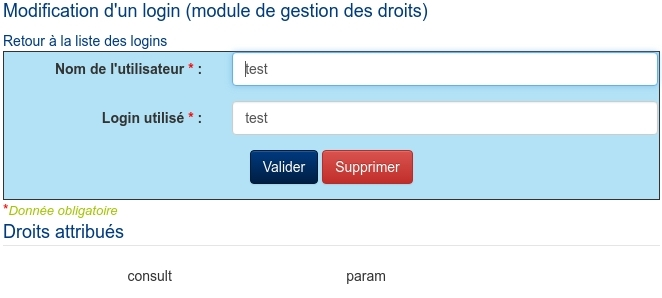
\includegraphics[width=\linewidth]{images/acl_login}
\caption{Écran de modification d'un login dans le module de gestion des droits}
\end{figure}


Sous l'écran de saisie figurent la liste des droits attribués à un login (en modification, le calcul n'est réalisé qu'à l'affichage de la page).

\subsection{Définir les groupes d'utilisateur}

Les groupes d'utilisateurs sont gérés selon un mécanisme d'héritage. Un groupe de haut niveau hérite des groupes précédents : si des droits ont été attribués à un groupe de niveau inférieur, un login associé à un groupe de niveau supérieur les récupère également.

Pour définir les groupes, dans le menu, choisissez \textit{Administration $\rightarrow$ ACL - groupes de logins}.

\begin{figure}[H]
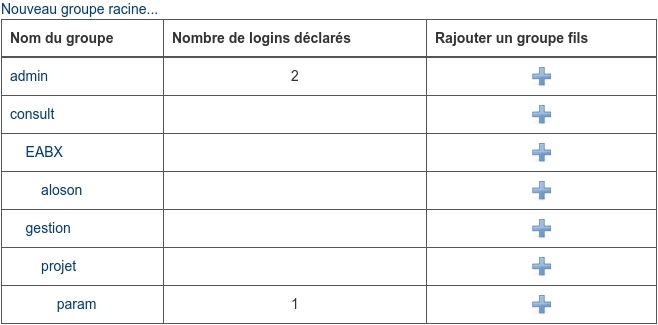
\includegraphics[width=\linewidth]{images/acl_groupe}
\caption{Liste des groupes de logins}
\end{figure}

Ainsi, le login déclaré dans le groupe \textit{param} récupérera les droits attribués aux groupes \textit{projet}, \textit{gestion} et \textit{consult}.

Pour créer un groupe, deux possibilités :
\begin{itemize}
\item soit le groupe est à la base d'une nouvelle branche : utilisez alors \textit{Nouveau groupe racine...} ;
\item soit le groupe hérite d'un autre groupe : cliquez sur le signe + (\textit{Rajouter un groupe fils}).
\end{itemize}

Vous pouvez indiquer les logins qui sont rattachés à ce groupe.


\subsection{Créer une application}
Le moteur utilisé pour faire fonctionner le logiciel COLLEC permet de gérer des droits différents pour des jeux de données différents, à partir du même code applicatif. Chaque couple \textit{logiciel} $\leftrightarrow$ \textit{base de données} constitue donc une \textit{application}, au sens de la gestion des droits.

Il est ainsi possible, à partir de la même base de données, de définir des droits différents selon les jeux de données utilisés (un jeu de données correspond à un schéma de base de données comprenant l'intégralité des tables applicatives).

À partir du menu, choisissez \textit{Administration $\rightarrow$ ACL - droits} :
\begin{figure}[H]
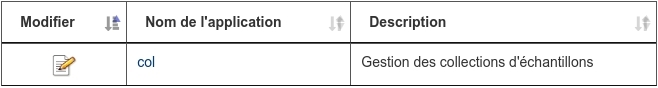
\includegraphics[width=\linewidth]{images/liste_appli}
\caption{Liste des applications déclarées}
\end{figure}

Pour créer une nouvelle application, choisissez \textit{Nouvelle application...}. 

\begin{figure}[H]
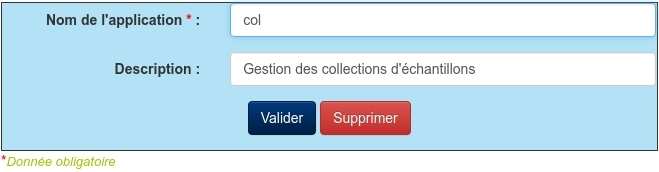
\includegraphics[width=\linewidth]{images/appli_change}
\caption{Écran de saisie d'une application}
\end{figure}

Le nom de l'application doit impérativement correspondre à la valeur \textit{\$GACL\_appli} dans les fichiers de paramètres : c'est ce qui permet au framework de savoir quels droits appliquer.

\subsection{Définir les droits utilisables dans l'application}

À partir de la liste des applications, cliquez sur le nom de celle pour laquelle vous voulez définir les droits utilisables. 
À partir de la liste, sélectionnez \textit{Nouveau droit...}.

\begin{figure}[H]
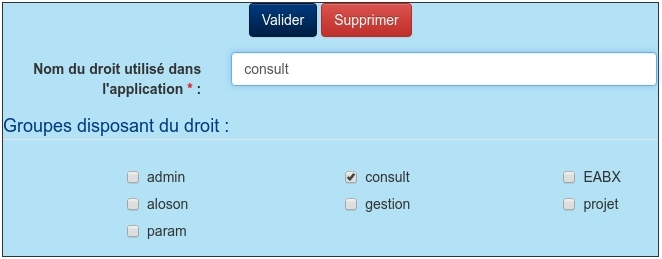
\includegraphics[width=\linewidth]{images/appli_droit}
\caption{Écran de saisie des droits associés à une application}
\label{applidroit}
\end{figure}

Le nom du droit doit être celui défini dans le corps de l'application (les droits sont positionnés dans les fichiers \textit{param/actions.xml}, qui contient la liste des modules utilisables, et \textit{param/menu.xml}, qui sert à générer le menu -- \textit{cf.} table \ref{droitsCollec} \textit{\nameref{droitsCollec}}, page \pageref{droitsCollec}).

Indiquez les groupes d'utilisateurs qui seront associés au droit courant.

\subsection{Cas particulier des groupes et des logins issus d'un annuaire LDAP}

Si vous avez paramétré l'application pour qu'elle s'appuie sur un annuaire LDAP pour gérer l'affectation des utilisateurs dans les groupes, vous n'êtes pas obligés de les déclarer explicitement dans le module de gestion des droits.

\subsubsection{Droits attribués à un groupe LDAP}

Tous les utilisateurs d'un groupe héritent d'un droit dans l'application.

\begin{itemize}
\item définissez le nom du groupe (en respectant la casse) dans le tableau des groupes d'utilisateurs (par exemple, EABX) ;
\item sélectionnez le nom de ce groupe dans les droits utilisables ;
\item tous les utilisateurs de l'annuaire LDAP récupéreront automatiquement les droits attribués à ce groupe.
\end{itemize}

\subsubsection{Droits attribués à un utilisateur particulier de l'annuaire LDAP}

Un utilisateur s'identifie auprès de l'annuaire LDAP, mais dispose de droits particuliers.

\begin{itemize}
\item créez son login dans la gestion des droits ;
\item rajoutez-le dans le groupe d'utilisateurs adéquat.
\end{itemize}


\section{Droits spécifiques de l'application COLLEC}

\subsection{Droits à positionner}
Voici les droits nécessaires pour faire fonctionner correctement l'application :

\begin{longtable}{|p{5cm}|p{10cm}|}
\hline
\textbf{Droit} & \textbf{Usage} \\
\hline
\endhead
admin &	Gestion des utilisateurs et des droits\\
\hline
param &	Définition des tables de paramètres généraux, gestion des collections\\
\hline
collection & rajout des types d'échantillons ou de conteneurs, import de masse \\
\hline
import & permet de réaliser des importations de masse \\
\hline
gestion &	Ajout d'un échantillon pour les projets autorisés, entrée/sortie. Droit attribué par défaut si l'utilisateur fait partie d'au moins un projet \\
\hline
consult	& Consultation des informations, sans possibilité de modification. Le droit de consultation doit être indiqué volontairement\\
\hline

\caption{\label{droitsCollec}Liste des droits utilisés}
\end{longtable}

Ces droits doivent être définis pour chaque application (couple \textit{logiciel} $\leftrightarrow$ \textit{base de données}) gérée par la base de gestion des droits.

\subsection{Gestion des collections}
\label{projet}

Les échantillons étant obligatoirement rattachés à une collcction, vous devrez en créer au minimum une à partir du menu de paramétrage. Un utilisateur avec les droits de gestion ne peut modifier que les échantillons pour lesquels il est autorisé (les collections qui sont rattachées au(x) groupe(s) dont il fait partie).

Voici le principe de gestion des droits pour les collections :
\begin{itemize}
\item Dans \textit{Administration} > \textit{ACL - Groupes de logins}, déclarez les groupes adéquats. En cas d'utilisation des groupes LDAP, les saisir avec la même casse que dans l'annuaire (EABX p. e.).

Il est possible de définir une hiérarchie des groupes, quelle que soit l'origine de l'affectation (base de données ou annuaire Ldap).
Dans le cas où l'annuaire Ldap n'est pas utilisé pour gérer les groupes, renseignez les logins en face des groupes dans le même écran ;
\item Dans les collections, sélectionnez les groupes autorisés (\textit{cf.} \ref{applidroit} \textit{\nameref{applidroit}}, page \pageref{applidroit}) ;
\item les utilisateurs faisant partie des groupes autorisés disposeront des droits de \textit{gestion} pour la collection considérée.
\end{itemize}

\section{Configurer les paramètres généraux}
\label{param}
L'ensemble des paramètres sont accessibles à partir du menu \textit{Paramètres}. 

Par défaut, tous les utilisateurs qui disposent du droit de consultation peuvent visualiser les paramètres. La modification n'est possible que pour ceux qui disposent des droits suivants :

\begin{longtable}{|p{4cm}|p{8cm}| p{3cm}|}
\hline
\textbf{Nom} & \textbf{Description} & \textbf{Droit nécessaire} \\
\hline
\endhead
Projets & Liste des projets et droits associés & admin \\
\hline
Protocoles & Protocoles de prélèvement des échantillons & collection \\
\hline
Opérations & Opérations rattachées aux protocoles & collection \\
\hline
Type d'événement & Événements survenant aux objets & param \\
\hline
Familles de conteneurs & Mécanisme pour retrouver les conteneurs selon leur nature (pièce, caisse...) & param, projet\\
\hline
Conditions de stockage & Mécanisme de conservation (lyophilisation, p. e.) & param, collection\\
\hline
Motifs de déstockage & Raisons invoquées pour sortir un objet du stock & param, collection\\
\hline
Types de conteneurs & Modèles de conteneurs (porteurs des étiquettes, entre autres) & param, collection\\
\hline
Statut des objets & Liste des statuts que peut prendre un objet & param\\
\hline
Type d'échantillon & Modèles des échantillons (rattachables à un type de conteneur) &  param, collection\\
\hline
Sous-échantillonnage & Pour les échantillons composés d'éléments non différenciables, unité utilisée pour réaliser le sous-échantillonnage (nombre, volume...) & param \\
\hline
Étiquettes & Modèles des étiquettes imprimables & param \\
\hline
Types d'identifiants & Types d'identifiants complémentaires des objets & param \\
\hline

\caption{Liste des paramètres et droits de modification associés}
\end{longtable}

\section{Créer ou modifier un modèle d'étiquettes}

\begin{figure}[H]
\centering
\fbox{
\includegraphics{images/etiquette}}
\caption{Exemple d'étiquette}
\end{figure}

Les étiquettes sont créées en recourant au logiciel FOP \cite{fop}, écrit en Java. Voici les opérations réalisées par l'application pour générer les étiquettes :
\begin{itemize}
\item pour chaque objet concerné (des containers ou des échantillons associés à un type de container, et si le type de container est rattaché à un modèle d'étiquettes), une image du QRcode est générée dans le dossier \textit{temp} ;
\item dans le dossier \textit{temp}, un fichier au format XML est généré, contenant les informations à imprimer sur l'étiquette ;
\item un fichier au format XSL, qui contient les ordres de création de l'étiquette, est également créé dans le même dossier. Le contenu de ce fichier est issu d'un enregistrement provenant de la table \textit{label} ;
\item le programme PHP fait appel à FOP pour générer, à partir du fichier XML et en utilisant le fichier XSL, un fichier PDF. Une page du fichier correspond à une étiquette (mécanisme utilisé par les imprimantes à étiquettes pour les séparer).
\end{itemize}

La configuration du modèle d'étiquettes revient à définir à la fois le contenu des informations qui seront insérées dans le QRCODE et la forme que prendra l'étiquette, c'est à dire les informations qui seront imprimées, le format, etc. Cette forme reprend la syntaxe XSL comprise par FOP.

\begin{figure}[H]

\includegraphics[width=\linewidth]{images/label}
\caption{Écran de saisie d'un modèle d'étiquette}
\end{figure}

\subsection{Définir le contenu du QRcode}
Le QRcode est un format de code barre normalisé en deux dimensions, qui permet de stocker jusqu'à 2000 caractères en 8 bits. 

Le principe retenu dans l'application est de stocker l'information au format JSON. Pour limiter la taille du code barre, les noms des balises doivent être les plus petites possibles. Voici les balises obligatoires à insérer systématiquement dans une étiquette :

\begin{longtable}{|p{3cm}|p{12cm}| }
\hline
\textbf{Nom} & \textbf{Description} \\
\hline
\endhead
uid & Identifiant unique de l'objet dans la base de données \\
\hline
db & Identifiant de la base de données. C'est la valeur du paramètre \textit{APPLI\_code} (\textit{cf.} \ref{paramspec} \textit{\nameref{paramspec}}, page \pageref{paramspec}) \\
\hline
\caption{Liste des balises à insérer obligatoirement dans les QRcodes}
\end{longtable}

D'autres informations peuvent être également insérées :
\begin{longtable}{|p{3cm}|p{12cm}| }
\hline
\textbf{Nom} & \textbf{Description} \\
\hline
\endhead
id & Identifiant métier principal (champ \textit{identifiant ou nom}, en saisie) \\
\hline
prj & Code de la collection (pour les échantillons) \\
\hline
clp & Code du risque associé au conteneur, en raison du produit de conservation utilisé \\
\hline
pn & Nom du protocole de collecte des échantillons \\
\hline
autres codes & tous les codes d'identification secondaires définis dans la table de paramètres \textit{Types d'identifiants} (\textit{cf.} \ref{param} \textit{\nameref{param}}, page \pageref{param}). \\
\hline
les champs utilisés dans les métadonnnées & les codes des champs utilisés dans la description des métadonnées. Un modèle d'étiquette ne peut être associé qu'à un type de métadonnées \\
\hline

\caption{Liste des balises facultatives insérables dans les QRcodes}
\end{longtable}

\subsection{Configuration du fichier XSL}

La syntaxe particulière du fichier XSL ne doit être modifiée qu'en conservant la version initiale (recopie dans un bloc-notes, par exemple), pour éviter de perdre une configuration opérationnelle suite à un mauvais paramétrage.

Voici la description du contenu du fichier et les zones modifiables.

\subsubsection{Entête du fichier}
Elle permet de modifier la taille de l'étiquette (largeur et hauteur maximale). Vous ne devriez changer que les attributs \textit{page-height} et \textit{page-width}. Pour les marges (attributs \textit{margin-}), soyez prudents et vérifiez notamment que les QRcodes ne soient pas rognés à cause de marges insuffisantes.

\begin{lstlisting}
<?xml version="1.0" encoding="utf-8"?>
<xsl:stylesheet version="1.0"
      xmlns:xsl="http://www.w3.org/1999/XSL/Transform"
      xmlns:fo="http://www.w3.org/1999/XSL/Format">
  <xsl:output method="xml" indent="yes"/>
  <xsl:template match="objects">
    <fo:root>
      <fo:layout-master-set>
        <fo:simple-page-master master-name="label"
              page-height="5cm" page-width="10cm" 
              margin-left="0.5cm" 
              margin-top="0.5cm" 
              margin-bottom="0cm" 
              margin-right="0.5cm">  
              <fo:region-body/>
        </fo:simple-page-master>
      </fo:layout-master-set>
      
      <fo:page-sequence master-reference="label">
         <fo:flow flow-name="xsl-region-body">        
          <fo:block>
          <xsl:apply-templates select="object" />
          </fo:block>

        </fo:flow>
      </fo:page-sequence>
    </fo:root>
   </xsl:template>
  <xsl:template match="object">
\end{lstlisting}

\subsubsection{Format de l'étiquette}
Le contenu de l'étiquette est décrit sous la forme d'un tableau (balises \textit{fo:table}). La première colonne contient le QRCode, la seconde le texte associé.

Ici, deux colonnes de taille identique (4 cm chacune) sont définies.

\begin{lstlisting}
  <fo:table table-layout="fixed" border-collapse="collapse"  
  border-style="none" width="8cm" 
  keep-together.within-page="always">
  <fo:table-column column-width="4cm"/>
  <fo:table-column column-width="4cm" />
 <fo:table-body  border-style="none" >
\end{lstlisting}

Les cellules (\textit{table-cell}) sont insérées dans une ligne (\textit{table-row}) :

\begin{lstlisting}
 	<fo:table-row>
\end{lstlisting}

\subsubsection{Insertion du QRcode}
Le QRcode est inséré dans un bloc. Les seules informations modifiables sont celles concernant la hauteur (attribut \textit{height} et la largeur (attribut \textit{content-width})). Veillez à ce que la hauteur et la largeur soient identiques, et ne modifiez pas les autres informations.

\begin{lstlisting}
  		<fo:table-cell> 
  		<fo:block>
  		<fo:external-graphic>
      <xsl:attribute name="src">
             <xsl:value-of select="concat(uid,'.png')" />
       </xsl:attribute>
       <xsl:attribute name="content-height">
       scale-to-fit
       </xsl:attribute>
       <xsl:attribute name="height">4cm</xsl:attribute>
        <xsl:attribute name="content-width">4cm</xsl:attribute>
        <xsl:attribute name="scaling">uniform</xsl:attribute>      
       </fo:external-graphic>
 		</fo:block>
   		</fo:table-cell>
\end{lstlisting}
\subsubsection{Contenu textuel}

Les autres informations sont affichées dans des blocs, avec une ligne par catégorie d'information.

L'étiquette commence ici par indiquer l'établissement (ici, IRSTEA), écrit en gras.

\begin{lstlisting}
  		<fo:table-cell>
		<fo:block>
			<fo:inline font-weight="bold">
				IRSTEA
			</fo:inline>
		</fo:block>
\end{lstlisting}

Chaque information est affichée dans un bloc, comprenant un titre (par exemple, \textit{uid}), associé à une ou plusieurs valeurs. Ainsi, la première ligne affiche sur la même ligne, et en gras (attribut \textit{font-weight="bold"}), le code de la base de données (\textit{<xsl:value-of select="db"/>}) et l'UID de l'objet (\textit{<xsl:value-of select="uid"/>}).

\begin{lstlisting}   		

  			<fo:block>uid:
  			<fo:inline font-weight="bold">
  			<xsl:value-of select="db"/>:
  			<xsl:value-of select="uid"/></fo:inline>
  			</fo:block>
  			<fo:block>id:
  			<fo:inline font-weight="bold"> 
  			<xsl:value-of select="id"/></fo:inline>
  			</fo:block>
  			<fo:block>prj:
  			<fo:inline font-weight="bold"> 
  			<xsl:value-of select="prj"/></fo:inline>
  			</fo:block>
  			<fo:block>clp:
  			<fo:inline font-weight="bold">
  			<xsl:value-of select="clp"/></fo:inline>
  			</fo:block>
\end{lstlisting}

\subsubsection{Fin de l'étiquette}

Une fois toutes les informations affichées, le tableau est fermé, et un saut de page est généré systématiquement :
\begin{lstlisting}
  		</fo:table-cell>
  	  	</fo:table-row>
  </fo:table-body>
  </fo:table>
   <fo:block page-break-after="always"/>
\end{lstlisting}

Enfin, le fichier XSL est correctement fermé :
\begin{lstlisting}
  </xsl:template>
</xsl:stylesheet>
\end{lstlisting}

Il est possible de créer des étiquettes avec des formats différents, par exemple en créant plusieurs lignes. Pensez à fermer vos balises, et qu'elles soient correctement imbriquées, pour éviter tout souci.

Pour aller plus loin dans la mise en page, consultez la documentation du projet FOP.

\section{Gestion des traces}

Tous les appels lancés par les utilisateurs vers les modules de l'application sont enregistrés dans la table \textit{gacl.log}, qui ne doit être accessible qu'aux personnes dûment autorisées. Les traces sont supprimées au bout d'un an (script de nettoyage exécuté lors de la connexion d'un utilisateur).

Voici un exemple de trace générée :
\begin{lstlisting}
log_id	login	nom_module	log_date	commentaire	ipaddress
523437	eric.quinton	col-Sample-write	2016-10-25 14:57:01	16	::1
523438	eric.quinton	col-sampleDisplay	2016-10-25 14:57:01	ok	::1
523436	eric.quinton	col-sampleWrite	2016-10-25 14:57:00	ok	::1
523435	eric.quinton	col-sampleChange	2016-10-25 14:56:58	ok	::1
523434	eric.quinton	col-sampleDisplay	2016-10-25 14:56:55	ok	::1
523433	eric.quinton	col-sampleList	2016-10-25 14:56:52	ok	::1
523431	eric.quinton	col-default	2016-10-25 14:53:05	ok	::1
523430	eric.quinton	col-connexion	2016-10-25 14:53:04	ldap-ok	::1
523429	unknown	col-connexion	2016-10-25 14:52:57	ok	::1
\end{lstlisting}

La colonne \textit{commentaire}, pour la ligne 523437, contient l'identifiant modifié (l'enregistrement 16 a été traité par le module sampleWrite -- Sample (majuscule du S) correspond au nom de la classe qui a été utilisée pour réaliser l'écriture vers la base de données). L'adresse IP est théoriquement celle de l'utilisateur (ici, connexion locale), y compris en prenant en compte le passage par un serveur Reverse-proxy\footnote{serveur mis en entrée du réseau privé, qui permet de masquer les adresses internes et de contrôler les accès depuis Internet}.

Parallèlement, les messages d'erreur sont envoyés au processus Linux SYSLOG, qui enregistre les traces dans le fichier \textit{/var/log/apache2/error.log}.

\chapter{Comment faire pour ?}
\section{Générer une liste d'échantillons vides}
Objectif : préparer des bocaux d'échantillons avant de partir en campagne de collecte. Ces bocaux doivent être étiquetés.

Le logiciel propose une procédure d'import de masse, qui permet de répondre à cette question.

Voici la méthode à utiliser :
\begin{itemize}
\item générez un fichier au format CSV (créé par exemple à partir de LibreOffice OpenDataSheet -- ODS), qui comprend une ligne par échantillon ;
\item lancez la procédure d'import : le programme vous indiquera les UID générés ;
\item recherchez les UID générés, et déclenchez l'impression des étiquettes.
\end{itemize}

\subsection{Structure du fichier CSV}

Toute opération d'import présente des risques : il est difficile de revenir en arrière une fois celle-ci terminée.
Pour les limiter, le logiciel va procéder en deux étapes. D'abord, la structure du fichier va être analysée, et la cohérence des informations indiquées vérifiée.
Ensuite, si aucune anomalie n'est détectée, l'import pourra être déclenché.

La première ligne du fichier doit comporter le nom des colonnes. Leur nom est normalisé et ne doit en aucun cas être modifié. Si une colonne n'existe pas, l'import du fichier sera rejeté.

Les identifiants numériques (\textit{project\_id} par exemple) doivent être recherchés dans les tables de paramètres de l'application.

Voici la liste des colonnes utilisables :
\begin{longtable}{|p{4cm}|p{8cm}| c|}
\hline
\textbf{Colonne} & \textbf{Description} & \textbf{Obligatoire} \\
\hline
\endhead
sample\_identifier & identifiant métier de l'échantillon & X \\
\hline
collection\_id & identifiant de la collection de rattachement & X \\
\hline
sample\_type\_id & identifiant du type d'échantillon & X \\
\hline
sample\_status\_id & identifiant du statut à attribuer & X \\
\hline
sampling\_place\_id & le numéro informatique de l'endroit où l'échantillon a été prélevé & \\
\hline
wgs84\_x & longitude GPS en WGS84 (degrés décimaux) & \\
\hline
wgs84\_y & latitude GPS en WGS84 (degrés décimaux) & \\
\hline
sampling\_date & date de création/échantillonnage de l'échantillon, au format dd/mm/yyyy & \\
\hline
expiration\_date & date d'expiration de l'échantillon, au format dd/mm/yyyy & \\
\hline
sample\_location & emplacement de rangement de l'échantillon dans le container (texte libre) & \\
\hline
sample\_column & n° de la colonne de stockage dans le container & \\
\hline
sample\_line & n° de la ligne de stockage dans le container & \\
\hline
sample\_multiple\_value & le nombre total de sous-échantillons (ou le volume total, ou le pourcentage...) contenu dans l'échantillon si le type d'échantillons utilisé le permet (valeur numérique, séparateur décimal : point) & \\
\hline
sample\_parent\_uid & UID du parent (création d'échantillons rattachés) &\\
\hline
sample\_metadata\_json & métadonnées rattachées à l'échantillon (au format json, p. e. : \{"taxon":"Alosa alosa"\}) & \\
\hline
container\_identifier & identifiant du container & X \\
\hline
container\_type\_id & identifiant du type de container & X \\
\hline
container\_status\_id & identifiant du statut à attribuer au container & \\
\hline
container\_column & n° de la colonne de stockage dans le container parent & \\
\hline
container\_line & n° de la ligne de stockage dans le container parent & \\
\hline
container\_parent\_uid & UID du container dans lequel le container courant est rangé & \\
\hline
identifiants complémentaires & une colonne par code supplémentaire (menu \textit{Paramètres $\rightarrow$ Types d'identifiants}) & \\
\hline

\caption{Liste des colonnes utilisables lors d'un import de masse}
\end{longtable}

Les champs obligatoires ne le sont que si l'identifiant de l'objet considéré -- échantillon ou container -- a été renseigné. Une ligne doit contenir au minimum soit un numéro d'échantillon, soit un numéro de container.

\subsection{Procédure d'import}

À partir du menu, choisissez \textit{Objet $\rightarrow$ import de masse}. Seuls les utilisateurs qui disposent du droit \textit{projet} ou \textit{import} pourront réaliser l'opération.
\begin{figure}[H]
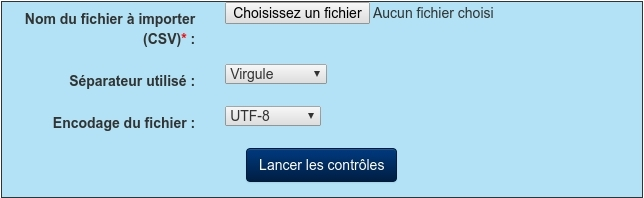
\includegraphics[width=\linewidth]{images/import_controle}
\caption{Sélection du fichier pour un import de masse}
\end{figure}

Sélectionnez le fichier à importer, vérifiez le séparateur utilisé. Préférez, si possible, les données au format UTF-8.

L'import sera réalisé ainsi :
\begin{enumerate}

\item  si sample\_identifier est renseigné : création de l'échantillon
\item    si container\_identifier est renseigné : création du container
\item    si container\_identifier et container\_parent\_uid sont renseignés : création du mouvement d'entrée du container
\item    si l'échantillon et le container ont été créés, création du mouvement d'entrée de l'échantillon dans le container
\item    si l'échantillon est créé, que container\_parent\_uid est renseigné, et que container\_identifier n'est pas rempli, création du mouvement d'entrée de l'échantillon dans le container indiqué

\end{enumerate}

Si des anomalies sont détectées lors du contrôle, un tableau récapitulant les problèmes rencontrés sera affiché, ressemblant à ceci :
\begin{figure}[H]
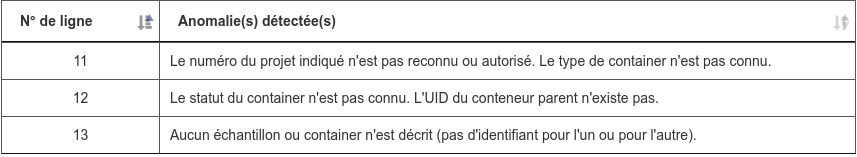
\includegraphics[width=\linewidth]{images/import_tableau}
\caption{Exemples d'anomalies détectées lors du contrôle de l'import}
\end{figure}

Si les contrôles se sont bien déroulés, le programme proposera alors de déclencher l'import, et affichera en retour les valeurs \textit{mini} et \textit{maxi} des UID générées.

\subsection{Autre usage}
Cette fonctionnalité peut également être utilisée pour déclencher l'import de listes d'échantillons pré-existants, et de créer automatiquement les mouvements adéquats pour les ranger dans leurs containers de stockage.

\subsection{Exemple de fichier}
\begin{figure}[H]
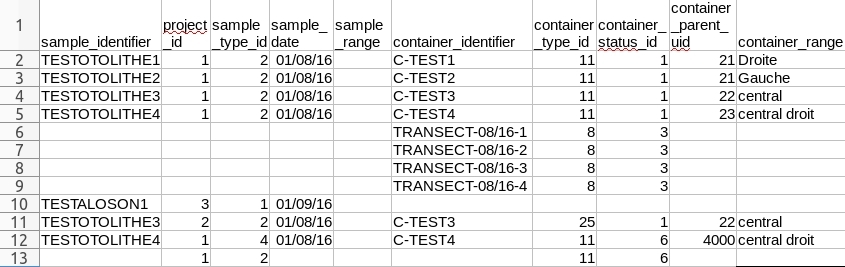
\includegraphics[width=\linewidth]{images/importcsv}
\caption{Exemple d'un fichier CSV}
\end{figure}

Dans cet exemple, l'import ne sera pas réalisé pour les raisons suivantes :
\begin{itemize}
\item en ligne 12, le numéro de container n'existe pas ;
\item la ligne 13 ne contient ni numéro d'échantillon, ni de numéro de container.
\end{itemize}

Sans tenir compte des erreurs, voici les opérations qui seraient exécutées :
\begin{itemize}
\item lignes 2 à 5, 11 et 12 : création d'échantillons, avec création du mouvement d'entrée dans les containers correspondants ;
\item lignes 6 à 9 : création de containers ;
\item ligne 10 : création d'un échantillon non rangé ;
\end{itemize}


%Annexes
\appendix

\section{Présentation}
L'objectif de ce chapitre est de présenter comment mettre en œuvre une réplication entre deux serveurs Postgresql, pour éviter toute perte accidentelle d'un enregistrement.

Il a été élaboré à partir de documents glanés sur le net : \cite{digitOcean}, 

Il a été réalisé par Alexandra Darrieutort, stagiaire à Irstea en 2016, et complété par Jacques Foury, responsable informatique du centre Irstea de Cestas (33).


\href{http://www.rassoc.com/gregr/weblog/2013/02/16/zero-to-postgresql-streaming-replication-in-10-mins/}{Zero to postgresql streaming replication in 10 mins}
\footnote{http://www.rassoc.com/gregr/weblog/2013/02/16/zero-to-postgresql-streaming-replication-in-10-mins/}

\href{http://connect.ed-diamond.com/GNU-Linux-Magazine/GLMF-184/Configurer-la-replication-d-un-serveur-PostgreSQL}{Configurer la replication d'un serveur PostgreSQL}
\footnote{http://connect.ed-diamond.com/GNU-Linux-Magazine/GLMF-184/Configurer-la-replication-d-un-serveur-PostgreSQL}

\href{https://wiki.postgresql.org/wiki/Binary_Replication_Tutorial}{Binary replication tutorial}
\footnote{https://wiki.postgresql.org/wiki/Binary_Replication_Tutorial}

\section{Besoins exprimés:}

Mise en place d'une réplication d'un serveur postgreSQL de sorte qu'il y ait préservation des données, c'est-à-dire qu'une écriture faite sur le serveur maître se retrouve sur le serveur esclave. Le besoin en haute disponibilité n'est pas primordial. 

\section{Principe:}

Le mode de réplication correspondant au besoin est \textit{maître/esclave}. On peut lire et écrire sur le maître et seulement lire sur l'esclave si il est configuré en \textit{hot standby}. Ici, le serveur maître est \textit{citerne-8} et le serveur esclave est \textit{chappie}.

Les modifications de données sont enregistrées dans des journaux de transactions appelés \textbf{WAL (Write-Ahead Log) xlogs}. Ces WAL sont transférés à l'esclave qui les rejoue continuellement de sorte à se retrouver dans le même état que le maître. Il sera alors prêt à prendre la relève en cas d'indisponibilité du maître.

Grâce au principe de \textit{Streaming replication}, on n'attend plus que le fichier WAL (16 Mio) soit rempli mais il sera transmis sans délai du maître à l'esclave.

\textcolor{Red}{Attention:}
\begin{itemize}
\item Dans la configuration, comme on va conserver 256 xlogs à l'aide du paramètre \textbf{wal\_keep\_segments}, il faut prévoir assez d'espace disque disponible.
\item La réplication entre deux serveurs de versions différentes de postgresql est impossible.
\end{itemize}

\newpage
\section{Mise à jour du serveur (version 9.3) en version 9.4 sur \textit{citerne-8:}}

On installe la dernière version de postgresql, on liste les clusters qui tournent et on supprime le cluster 9.4 existant:

\smallskip
\begin{Verbatim}[frame=single,framerule=1mm,framesep=3mm,rulecolor=\color{brown}]
root@citerne-8:~# apt-get install postgresql-9.4
root@citerne-8:~# pg_lsclusters
root@citerne-8:~# pg_dropcluster --stop 9.4 main
\end{Verbatim}


\vspace{2mm}

Mise à jour du cluster:
\smallskip
\begin{Verbatim}[frame=single,framerule=1mm,framesep=3mm,rulecolor=\color{brown}]
root@citerne-8:~# pg_upgradecluster 9.3 main 
\end{Verbatim}

\vspace{2mm}

Donne la liste des clusters et dit s'ils sont actifs ou non: 
\smallskip
\begin{Verbatim}[frame=single,framerule=1mm,framesep=3mm,rulecolor=\color{brown}]
root@citerne-8:~# pg_lsclusters
root@citerne-8:~# pg_dropcluster --stop 9.3 main
\end{Verbatim}

\vspace{2mm}

On supprime le cluster de version 9.3:
\smallskip
\begin{Verbatim}[frame=single,framerule=1mm,framesep=3mm,rulecolor=\color{brown}]
root@citerne-8:~# pg_dropcluster --stop 9.3 main 
\end{Verbatim}

\vspace{2mm}

Et on modifie le port du cluster 9.4 dans le fichier \textit{/etc/postgresql/9.4/main/postgresql.conf}:
\smallskip
\begin{Verbatim}[frame=single,framerule=1mm,framesep=3mm,rulecolor=\color{brown}]
port = 5432
\end{Verbatim}

\section{Installation de postgreSQL sur \textit{chappie} et mise en place des clés ssh:}

\bigskip
\begin{Verbatim}[frame=single,framerule=1mm,framesep=3mm,rulecolor=\color{brown}]
root@chappie:~# apt-get install postgresql-9.4
root@chappie:~# su - postgres
postgres@chappie:~$ mkdir /var/lib/postgresql/.ssh/
postgres@chappie:~$ ssh-keygen
\end{Verbatim}

Pour la connexion ssh entre les deux serveurs, il faut mettre la clé de l'utilisateur postgres contenue dans le fichier \textbf{id\_rsa.pub} sur \textit{chappie} dans le fichier \textbf{authorized\_keys} de \textit{citerne-8} et inversement.

\section{Mise en place de la réplication:}

\subsection{\textcolor{Firebrick3}{\Large Maître}}

Création de l'utilisateur prosgresql chargé de la réplication:
\smallskip
\begin{Verbatim}[frame=single,framerule=1mm,framesep=3mm,rulecolor=\color{brown}]
root@citerne-8:~# su - postgres
postgres:~$ psql -c "CREATE USER rep REPLICATION LOGIN ENCRYPTED PASSWORD 'desperados';"
\end{Verbatim}

\vspace{2mm}

Dans le fichier \textbf{pg\_hba.conf} (\textit{/etc/postgresql/9.4/main/}) ajouter:
\smallskip
\begin{Verbatim}[frame=single,framerule=1mm,framesep=3mm,rulecolor=\color{brown}]
host    replication     rep     10.33.192.31/32   md5
\end{Verbatim}

\vspace{2mm}

Pour le paramètre \textbf{wal\_keep\_segments}, on lui donne une valeur assez grande pour éviter d'accumuler un retard trop important entre les deux serveurs en cas d'indisponibilité de l'esclave.

Dans le fichier \textbf{postgresql.conf} ajouter ces lignes:

\textit{Attention: Si vous faites un copier-coller, les apostrophes ne sont pas des apostrophes droites donc il faudra les modifier.}
\smallskip
\begin{Verbatim}[frame=single,framerule=1mm,framesep=3mm,rulecolor=\color{brown}]
listen_address = 'localhost,10.33.192.36' 
wal_level = hot_standby 
max_wal_senders = 3 
max_wal_size = 436MB 
wal_keep_segments = 256 
\end{Verbatim}

Ensuite, on redémarre le service postgresql.

\vspace{2mm}

\subsection{\textcolor{Firebrick3}{\Large Esclave}}

On arrête le service postgresql.

\vspace{2mm}

On ajoute ces lignes dans le fichier \textbf{postgresql.conf}:
\smallskip
\begin{Verbatim}[frame=single,framerule=1mm,framesep=3mm,rulecolor=\color{brown}]
wal_level = hot_standby
max_wal_senders = 3
max_wal_size = 384MB
wal_keep_segments = 256
hot_standby = on
max_locks_per_transaction = 128
\end{Verbatim}

\vspace{2mm}

Dans le fichier \textbf{pg\_hba.conf}:
\smallskip
\begin{Verbatim}[frame=single,framerule=1mm,framesep=3mm,rulecolor=\color{brown}]
host    replication     rep     10.33.192.36/32 md5 
\end{Verbatim}

\vspace{2mm}

On effectue la sauvegarde complète des bases sous l'utilisateur postgres:

\smallskip
\begin{Verbatim}[frame=single,framerule=1mm,framesep=3mm,rulecolor=\color{brown}]
pg_dropcluster 9.5 main
pg_basebackup -h 10.33.192.36 -D /var/lib/postgresql/9.5/main -U rep -v -P --xlog
\end{Verbatim}
On ajoute l'option - -xlog pour garder les derniers journaux de transactions.

\vspace{2mm}

On crée le fichier \textbf{recovery.conf} dans \textit{/var/lib/postgresql/9.5/main/} et on y configure la restauration continue.

La restauration en continu s'active à l'aide du paramètre \textit{standby\_mode}. Pour se connecter au maître et récupérer les WAL, on définit les informations nécessaires dans le paramètre \textit{primary\_conninfo}. Et enfin, pour arrêter la restauration, il faut créer le \textit{trigger\_file}.
\smallskip
\begin{Verbatim}[frame=single,framerule=1mm,framesep=3mm,rulecolor=\color{brown}]
standby_mode = on 
primary_conninfo = 'host=10.33.192.36 port=5432 user=rep password=desperados' 
trigger_file = '/var/lib/postgresql/9.4/postgresql.trigger' 
\end{Verbatim}

Pour finir on démarre le service postgresql.

\section{Informations de monitoring:}

Le fichier de logs \textbf{postgresql-9.4-main.log} se trouve dans le répertoire \textit{/var/log/postgresql/}

\vspace{4mm}

Pour savoir où en est la réplication du côté du maître:
\smallskip
\begin{Verbatim}[frame=single,framerule=1mm,framesep=3mm,rulecolor=\color{brown}]
sudo -u postgres psql -x -c "select * from pg_stat_replication;"
\end{Verbatim}

\vspace{4mm}

Pour savoir depuis quand remonte la dernière synchronisation du côté de l'esclave:
\smallskip
\begin{Verbatim}[frame=single,framerule=1mm,framesep=3mm,rulecolor=\color{brown}]
sudo -u postgres psql -x -c "SELECT now() - pg_last_xact_replay_timestamp() AS time_lag;"
\end{Verbatim}

\vspace{4mm}

Pour voir le numéro du snapshot actuelle:
\smallskip
\begin{Verbatim}[frame=single,framerule=1mm,framesep=3mm,rulecolor=\color{brown}]
sudo -u postgres psql -x -c "SELECT txid_current_snapshot();"
\end{Verbatim}

\section{Pour tester le failover:}

Le serveur maître est indisponible, on va arrêter la restauration continue sur l'esclave, pour qu'il devienne le maître, en créant le fichier trigger. Les bases vont alors passer en mode read/write et le fichier \textit{recovery.conf} sera renommé \textit{recovery.done}.
\smallskip
\begin{Verbatim}[frame=single,framerule=1mm,framesep=3mm,rulecolor=\color{brown}]
sudo touch /var/lib/postgresql/9.4/postgresql.trigger
\end{Verbatim}

Ensuite, lorsque le maître sera de retour, la réplication ne fonctionnera plus. Il faudra recommencer ces étapes sur l'esclave pour que la réplication se remette en marche.

\smallskip
\begin{Verbatim}[frame=single,framerule=1mm,framesep=3mm,rulecolor=\color{brown}]
service postgresql stop
rm -rf /var/lib/postgresql/9.4/main/
pg_basebackup -h 10.33.192.36 -D /var/lib/postgresql/9.4/main -U rep -v -P --xlog
\end{Verbatim}

Ensuite, il faut recréer le fichier recovery.conf comme dans la \textit{partie 5.2} et on démarre le service.


\chapter{Structure de la base de données}

La structure et le détail des tables peut être consulté directement depuis le menu \textit{Paramètres} de l'application.

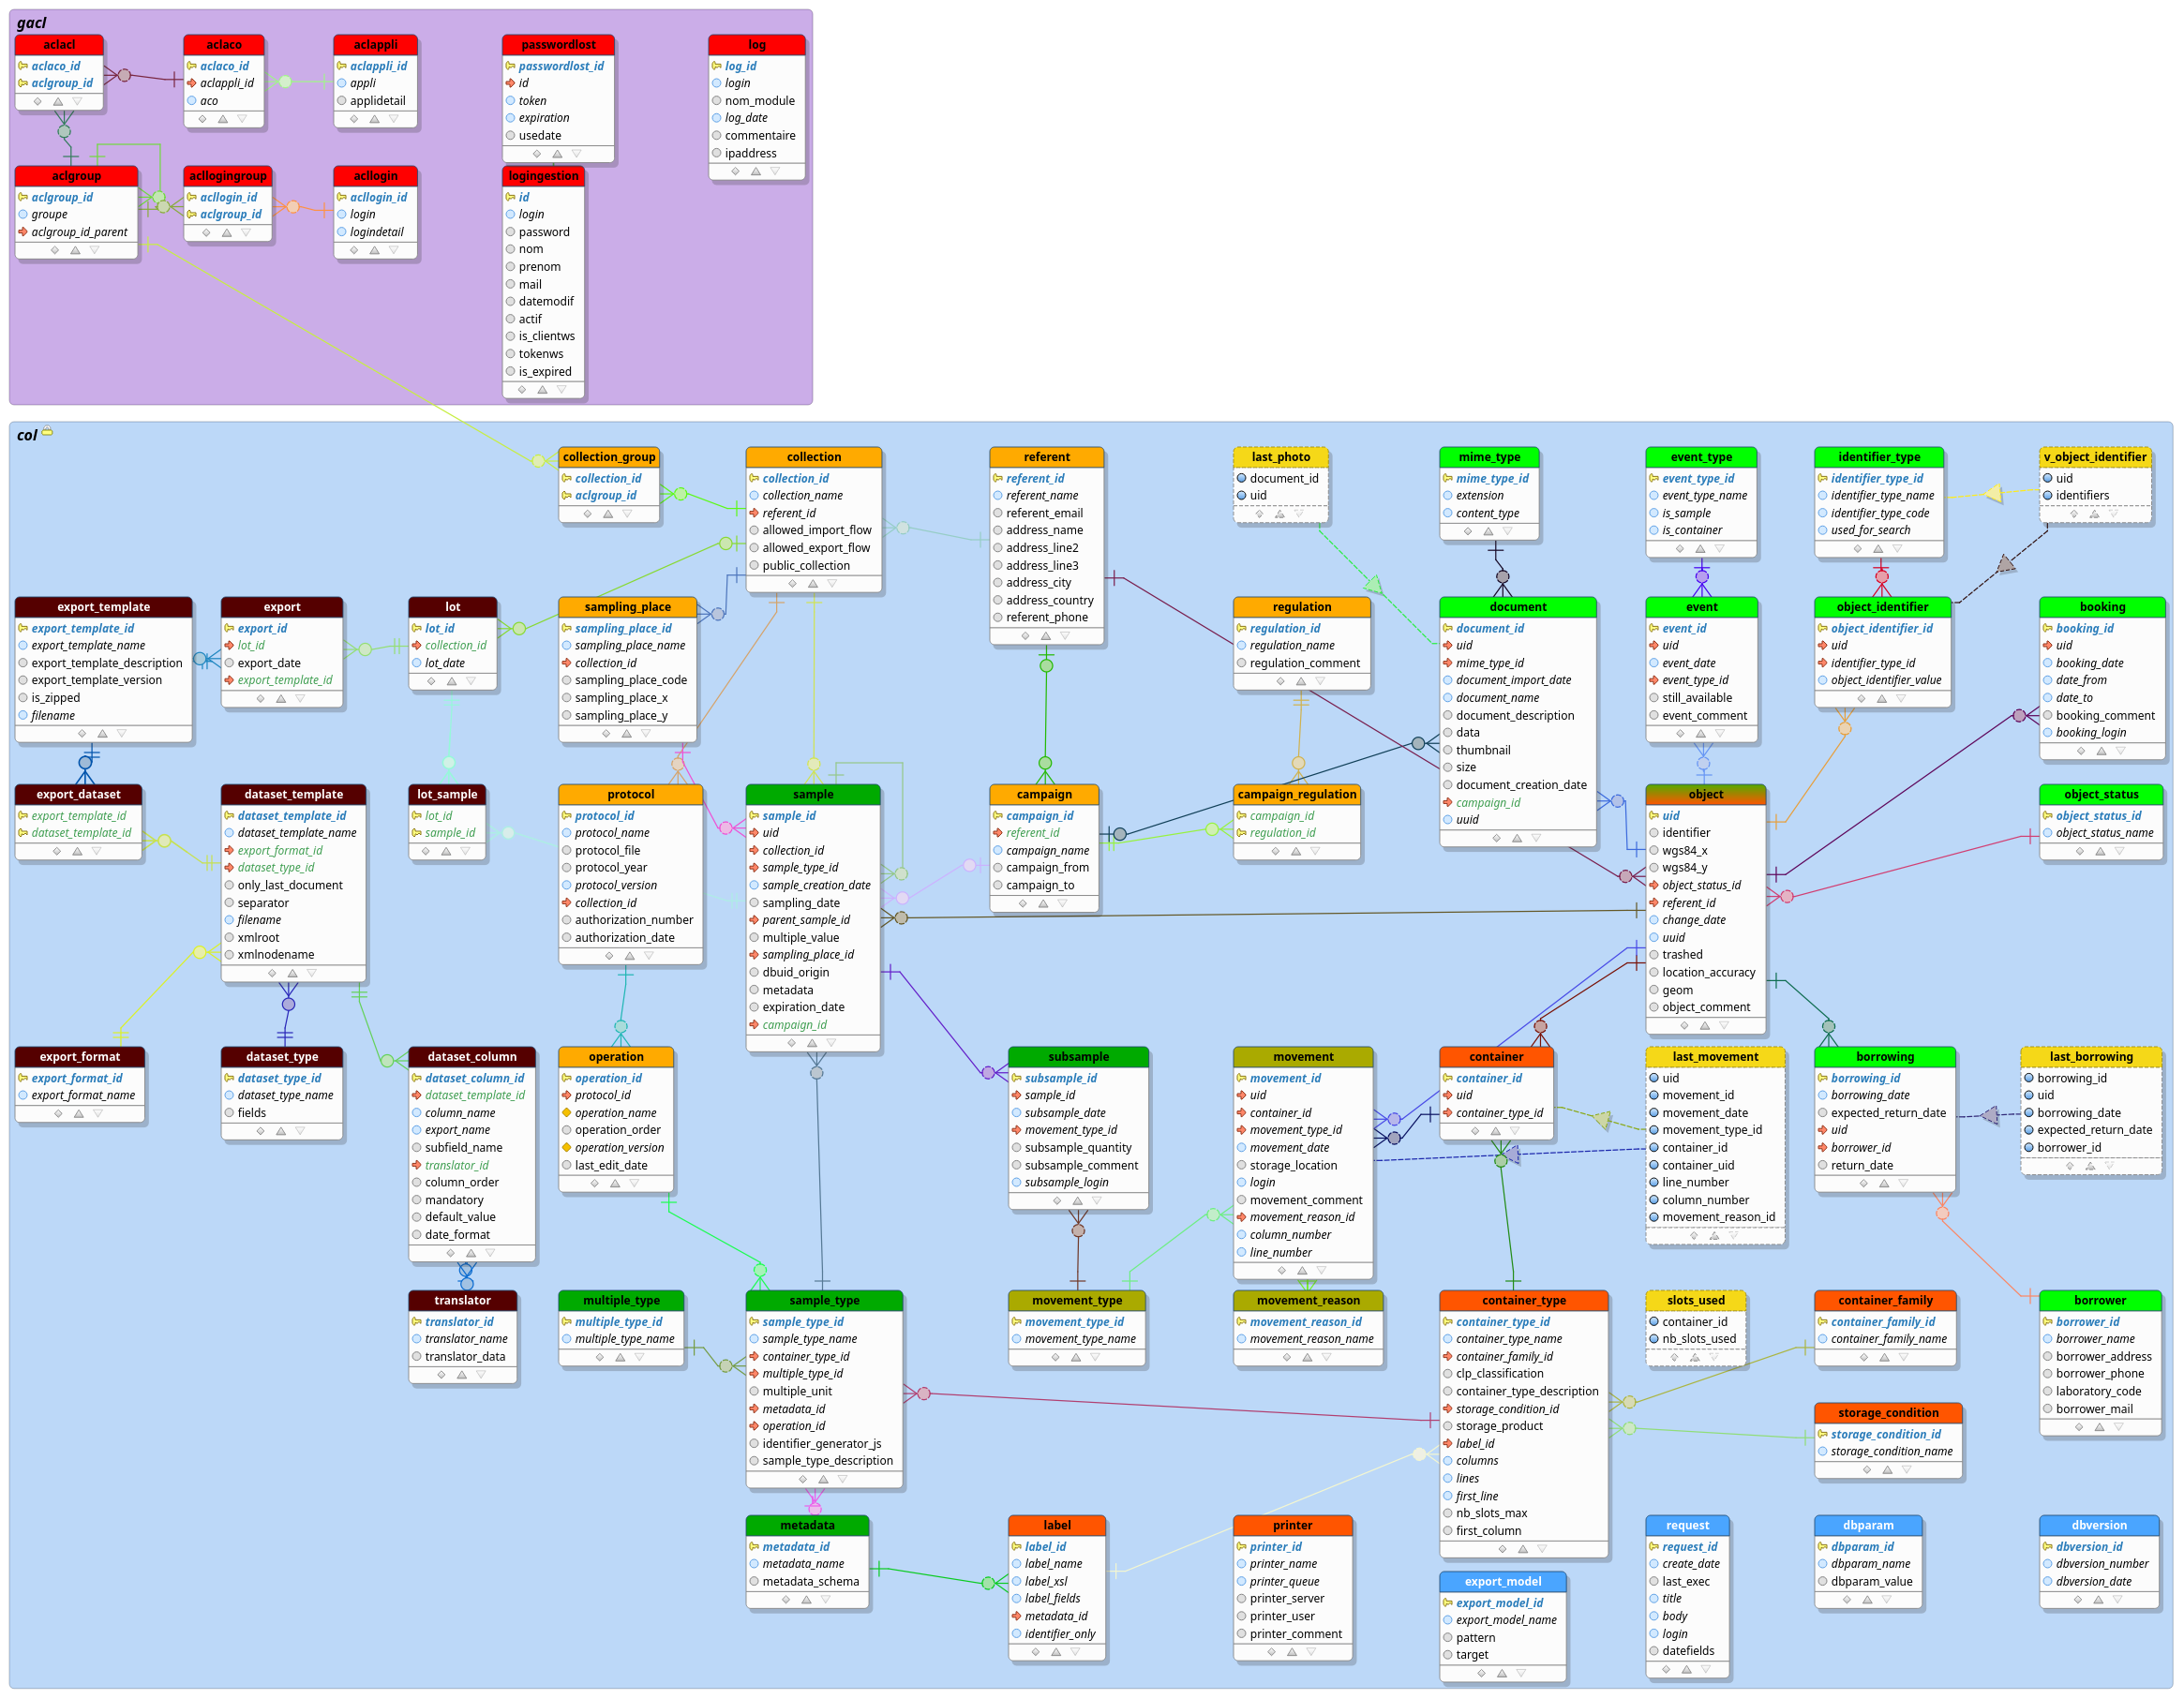
\includegraphics[
width=\textwidth
%angle=90
]{../collec-schema}


\section{Description des tables}
\subsection{booking}
Table des réservations d'objets

\begin{tabular}{|l| p{2cm}|c|c|c| p{3cm}|}
\hline
Column name & Type & Not null & Key & Foreign key & Comment \\
\hline
booking\_id & integer & X & X & & \\
\hline
uid & integer & X & & X & \\
\hline
booking\_date & timestamp without time zone & X & & & Date de la réservation\\
\hline
date\_from & timestamp without time zone & X & & & Date-heure de début de la réservation\\
\hline
date\_to & timestamp without time zone & X & & & Date-heure de fin de la réservation\\
\hline
booking\_comment & character varying & & & & Commentaire\\
\hline
booking\_login & character varying & X & & & Compte ayant réalisé la réservation\\
\hline
\end{tabular}
\subsection{container}
Liste des conteneurs d'échantillon

\begin{tabular}{|l| p{2cm}|c|c|c| p{3cm}|}
\hline
Column name & Type & Not null & Key & Foreign key & Comment \\
\hline
container\_id & integer & X & X & & \\
\hline
uid & integer & X & & X & \\
\hline
container\_type\_id & integer & X & & X & \\
\hline
\end{tabular}
\subsection{container\_family}
Famille générique des conteneurs

\begin{tabular}{|l| p{2cm}|c|c|c| p{3cm}|}
\hline
Column name & Type & Not null & Key & Foreign key & Comment \\
\hline
container\_family\_id & integer & X & X & & \\
\hline
container\_family\_name & character varying & X & & & \\
\hline
is\_movable & boolean & X & & & Indique si la famille de conteneurs est déplçable facilement ou non (éprouvette : oui, armoire : non)\\
\hline
\end{tabular}
\subsection{container\_type}
Table des types de conteneurs

\begin{tabular}{|l| p{2cm}|c|c|c| p{3cm}|}
\hline
Column name & Type & Not null & Key & Foreign key & Comment \\
\hline
container\_type\_id & integer & X & X & & \\
\hline
container\_type\_name & character varying & X & & & \\
\hline
container\_family\_id & integer & X & & X & \\
\hline
clp\_classification & character varying & & & & Classification du risque conformément à la directive européenne CLP\\
\hline
label\_id & integer & & & X & \\
\hline
container\_type\_description & character varying & & & & Description longue\\
\hline
storage\_condition\_id & integer & & & X & \\
\hline
storage\_product & character varying & & & & Produit utilisé pour le stockage (formol, alcool...)\\
\hline
columns & integer & X & & & Nombre de colonnes de stockage dans le container\\
\hline
lines & integer & X & & & Nombre de lignes de stockage dans le container\\
\hline
first\_line & character varying & X & & & T : top, premiere ligne en haut B: bottom, premiere ligne en bas\\
\hline
\end{tabular}
\subsection{document}
Documents numériques rattachés à un poisson ou à un événement

\begin{tabular}{|l| p{2cm}|c|c|c| p{3cm}|}
\hline
Column name & Type & Not null & Key & Foreign key & Comment \\
\hline
document\_id & integer & X & X & & \\
\hline
uid & integer & X & & X & \\
\hline
mime\_type\_id & integer & X & & X & \\
\hline
document\_import\_date & timestamp without time zone & X & & & Date d'import dans la base de données\\
\hline
document\_name & character varying & X & & & Nom d'origine du document\\
\hline
document\_description & character varying & & & & Description libre du document\\
\hline
data & bytea & & & & Contenu du document\\
\hline
thumbnail & bytea & & & & Vignette au format PNG (documents pdf, jpg ou png)\\
\hline
size & integer & & & & Taille du fichier téléchargé\\
\hline
document\_creation\_date & timestamp without time zone & & & & Date de création du document (date de prise de vue de la photo)\\
\hline
\end{tabular}
\subsection{event}
Table des événements

\begin{tabular}{|l| p{2cm}|c|c|c| p{3cm}|}
\hline
Column name & Type & Not null & Key & Foreign key & Comment \\
\hline
event\_id & integer & X & X & & \\
\hline
uid & integer & X & & X & \\
\hline
event\_date & timestamp without time zone & X & & & Date / heure de l'événement\\
\hline
event\_type\_id & integer & X & & X & \\
\hline
still\_available & character varying & & & & définit ce qu'il reste de disponible dans l'objet\\
\hline
event\_comment & character varying & & & & \\
\hline
\end{tabular}
\subsection{event\_type}
Types d'événement

\begin{tabular}{|l| p{2cm}|c|c|c| p{3cm}|}
\hline
Column name & Type & Not null & Key & Foreign key & Comment \\
\hline
event\_type\_id & integer & X & X & & \\
\hline
event\_type\_name & character varying & X & & & \\
\hline
is\_sample & boolean & X & & & L'événement s'applique aux échantillons\\
\hline
is\_container & boolean & X & & & L'événement s'applique aux conteneurs\\
\hline
\end{tabular}
\subsection{identifier\_type}
Table des types d'identifiants

\begin{tabular}{|l| p{2cm}|c|c|c| p{3cm}|}
\hline
Column name & Type & Not null & Key & Foreign key & Comment \\
\hline
identifier\_type\_id & integer & X & X & & \\
\hline
identifier\_type\_name & character varying & X & & & Nom textuel de l'identifiant\\
\hline
identifier\_type\_code & character varying & X & & & Code utilisé pour la génération des étiquettes\\
\hline
used\_for\_search & boolean & X & & & Indique si l'identifiant doit être utilise pour les recherches a partir des codes-barres\\
\hline
\end{tabular}
\subsection{label}
Table des modèles d'étiquettes

\begin{tabular}{|l| p{2cm}|c|c|c| p{3cm}|}
\hline
Column name & Type & Not null & Key & Foreign key & Comment \\
\hline
label\_id & integer & X & X & & \\
\hline
label\_name & character varying & X & & & Nom du modèle\\
\hline
label\_xsl & character varying & X & & & Contenu du fichier XSL utilisé pour la transformation FOP (https://xmlgraphics.apache.org/fop/)\\
\hline
label\_fields & character varying & X & & & Liste des champs à intégrer dans le QRCODE, séparés par une virgule\\
\hline
metadata\_id & integer & & & X & \\
\hline
identifier\_only & boolean & X & & & true : le qrcode ne contient qu'un identifiant metier\\
\hline
\end{tabular}
\subsection{mime\_type}
Types mime des fichiers importés

\begin{tabular}{|l| p{2cm}|c|c|c| p{3cm}|}
\hline
Column name & Type & Not null & Key & Foreign key & Comment \\
\hline
mime\_type\_id & integer & X & X & & \\
\hline
extension & character varying & X & & & Extension du fichier correspondant\\
\hline
content\_type & character varying & X & & & type mime officiel\\
\hline
\end{tabular}
\subsection{movement\_type}
Type de mouvement

\begin{tabular}{|l| p{2cm}|c|c|c| p{3cm}|}
\hline
Column name & Type & Not null & Key & Foreign key & Comment \\
\hline
movement\_type\_id & integer & X & X & & \\
\hline
movement\_type\_name & character varying & X & & & \\
\hline
\end{tabular}
\subsection{multiple\_type}
Table des types de contenus multiples

\begin{tabular}{|l| p{2cm}|c|c|c| p{3cm}|}
\hline
Column name & Type & Not null & Key & Foreign key & Comment \\
\hline
multiple\_type\_id & integer & X & X & & \\
\hline
multiple\_type\_name & character varying & X & & & \\
\hline
\end{tabular}
\subsection{object}
Table des objets Contient les identifiants génériques

\begin{tabular}{|l| p{2cm}|c|c|c| p{3cm}|}
\hline
Column name & Type & Not null & Key & Foreign key & Comment \\
\hline
uid & integer & X & X & & \\
\hline
identifier & character varying & & & & Identifiant fourni le cas échéant par le projet\\
\hline
object\_status\_id & integer & & & X & \\
\hline
wgs84\_x & double precision & & & & Longitude GPS, en valeur décimale\\
\hline
wgs84\_y & double precision & & & & Latitude GPS, en valeur décimale\\
\hline
referent\_id & integer & & & X & \\
\hline
\end{tabular}
\subsection{object\_identifier}
Table des identifiants complémentaires normalisés

\begin{tabular}{|l| p{2cm}|c|c|c| p{3cm}|}
\hline
Column name & Type & Not null & Key & Foreign key & Comment \\
\hline
object\_identifier\_id & integer & X & X & & \\
\hline
uid & integer & X & & X & \\
\hline
identifier\_type\_id & integer & X & & X & \\
\hline
object\_identifier\_value & character varying & X & & & Valeur de l'identifiant\\
\hline
\end{tabular}
\subsection{object\_status}
Table des statuts possibles des objets

\begin{tabular}{|l| p{2cm}|c|c|c| p{3cm}|}
\hline
Column name & Type & Not null & Key & Foreign key & Comment \\
\hline
object\_status\_id & integer & X & X & & \\
\hline
object\_status\_name & character varying & X & & & \\
\hline
\end{tabular}
\subsection{collection\_group}
Table des autorisations d'accès à un projet

\begin{tabular}{|l| p{2cm}|c|c|c| p{3cm}|}
\hline
Column name & Type & Not null & Key & Foreign key & Comment \\
\hline
collection\_id & integer & X & X & X & \\
\hline
aclgroup\_id & integer & X & X & X & \\
\hline
\end{tabular}
\subsection{sample}
Table des échantillons

\begin{tabular}{|l| p{2cm}|c|c|c| p{3cm}|}
\hline
Column name & Type & Not null & Key & Foreign key & Comment \\
\hline
sample\_id & integer & X & X & & \\
\hline
uid & integer & X & & X & \\
\hline
project\_id & integer & X & & X & \\
\hline
collection\_id & integer & X & & X & \\
\hline
sample\_type\_id & integer & X & & X & \\
\hline
sample\_creation\_date & timestamp without time zone & X & & & Date de création de l'enregistrement dans la base de données\\
\hline
sample\_date & timestamp without time zone & & & & Date de création de l'échantillon physique\\
\hline
sampling\_date & timestamp without time zone & & & & Date de création de l'échantillon physique\\
\hline
parent\_sample\_id & integer & & & X & \\
\hline
multiple\_value & double precision & & & & Nombre initial de sous-échantillons\\
\hline
sampling\_place\_id & integer & & & X & \\
\hline
dbuid\_origin & character varying & & & & référence utilisée dans la base de données d'origine, sous la forme db:uid Utilisé pour lire les étiquettes créées dans d'autres instances\\
\hline
metadata & json & & & & Metadonnees associees de l'echantillon\\
\hline
expiration\_date & timestamp without time zone & & & & \\
\hline
\end{tabular}
\subsection{sample\_type}
Types d'échantillons

\begin{tabular}{|l| p{2cm}|c|c|c| p{3cm}|}
\hline
Column name & Type & Not null & Key & Foreign key & Comment \\
\hline
sample\_type\_id & integer & X & X & & \\
\hline
sample\_type\_name & character varying & X & & & \\
\hline
container\_type\_id & integer & & & X & \\
\hline
multiple\_type\_id & integer & & & X & \\
\hline
multiple\_unit & character varying & & & & Unité caractérisant le sous-échantillon\\
\hline
metadata\_id & integer & & & X & \\
\hline
operation\_id & integer & & & X & \\
\hline
identifier\_generator\_js & character varying & & & & Champ comprenant le code de la fonction javascript permettant de générer automatiquement un identifiant à partir des informations saisies\\
\hline
\end{tabular}
\subsection{storage\_condition}
Condition de stockage

\begin{tabular}{|l| p{2cm}|c|c|c| p{3cm}|}
\hline
Column name & Type & Not null & Key & Foreign key & Comment \\
\hline
storage\_condition\_id & integer & X & X & & \\
\hline
storage\_condition\_name & character varying & X & & & \\
\hline
\end{tabular}
\subsection{subsample}
Table des prélèvements et restitutions de sous-échantillons

\begin{tabular}{|l| p{2cm}|c|c|c| p{3cm}|}
\hline
Column name & Type & Not null & Key & Foreign key & Comment \\
\hline
subsample\_id & integer & X & X & & \\
\hline
sample\_id & integer & X & & X & \\
\hline
subsample\_date & timestamp without time zone & X & & & Date/heure de l'opération\\
\hline
movement\_type\_id & integer & X & & X & \\
\hline
subsample\_quantity & double precision & & & & Quantité prélevée ou restituée\\
\hline
subsample\_comment & character varying & & & & \\
\hline
subsample\_login & character varying & X & & & Login de l'utilisateur ayant réalisé l'opération\\
\hline
\end{tabular}
\subsection{sampling\_place}
Table des lieux génériques d'échantillonnage

\begin{tabular}{|l| p{2cm}|c|c|c| p{3cm}|}
\hline
Column name & Type & Not null & Key & Foreign key & Comment \\
\hline
sampling\_place\_id & integer & X & X & & \\
\hline
sampling\_place\_name & character varying & X & & & \\
\hline
collection\_id & integer & & & X & \\
\hline
sampling\_place\_code & character varying & & & & Code métier de la station\\
\hline
sampling\_place\_x & double precision & & & & Longitude de la station, en WGS84\\
\hline
sampling\_place\_y & double precision & & & & Latitude de la station, en WGS84\\
\hline
\end{tabular}
\subsection{dbversion}
Table des versions de la base de donnees

\begin{tabular}{|l| p{2cm}|c|c|c| p{3cm}|}
\hline
Column name & Type & Not null & Key & Foreign key & Comment \\
\hline
dbversion\_id & integer & X & X & & \\
\hline
dbversion\_number & character varying & X & & & Numero de la version\\
\hline
dbversion\_date & timestamp without time zone & X & & & Date de la version\\
\hline
\end{tabular}
\subsection{movement\_reason}
List of the reasons of the movement

\begin{tabular}{|l| p{2cm}|c|c|c| p{3cm}|}
\hline
Column name & Type & Not null & Key & Foreign key & Comment \\
\hline
movement\_reason\_id & integer & X & X & & \\
\hline
movement\_reason\_name & character varying & X & & & \\
\hline
\end{tabular}
\subsection{printer}
Table des imprimantes gerees directement par le serveur

\begin{tabular}{|l| p{2cm}|c|c|c| p{3cm}|}
\hline
Column name & Type & Not null & Key & Foreign key & Comment \\
\hline
printer\_id & integer & X & X & & \\
\hline
printer\_name & character varying & X & & & Nom general de l'imprimante, affiche dans les masques de saisie\\
\hline
printer\_queue & character varying & X & & & Nom de l'imprimante telle qu'elle est connue par le systeme\\
\hline
printer\_server & character varying & & & & Adresse du serveur, si imprimante non locale\\
\hline
printer\_user & character varying & & & & Utilisateur autorise a imprimer \\
\hline
printer\_comment & character varying & & & & Commentaire\\
\hline
\end{tabular}
\subsection{movement}
Records of objects movements

\begin{tabular}{|l| p{2cm}|c|c|c| p{3cm}|}
\hline
Column name & Type & Not null & Key & Foreign key & Comment \\
\hline
movement\_id & integer & X & X & & \\
\hline
uid & integer & X & & X & \\
\hline
container\_id & integer & & & X & \\
\hline
movement\_type\_id & integer & X & & X & \\
\hline
movement\_date & timestamp without time zone & X & & & Date/heure du mouvement\\
\hline
storage\_location & character varying & & & & Emplacement de l'échantillon dans le conteneur\\
\hline
login & character varying & X & & & Nom de l'utilisateur ayant réalisé l'opération\\
\hline
movement\_comment & character varying & & & & Commentaire\\
\hline
movement\_reason\_id & integer & & & X & \\
\hline
column\_number & integer & X & & & No de la colonne de stockage dans le container\\
\hline
line\_number & integer & X & & & No de la ligne de stockage dans le container\\
\hline
\end{tabular}
\subsection{collection}
List of all collections into the database

\begin{tabular}{|l| p{2cm}|c|c|c| p{3cm}|}
\hline
Column name & Type & Not null & Key & Foreign key & Comment \\
\hline
collection\_id & integer & X & X & & \\
\hline
collection\_name & character varying & X & & & \\
\hline
referent\_id & integer & & & X & \\
\hline
\end{tabular}
\subsection{metadata}
Table des metadata utilisables dans les types d'echantillons

\begin{tabular}{|l| p{2cm}|c|c|c| p{3cm}|}
\hline
Column name & Type & Not null & Key & Foreign key & Comment \\
\hline
metadata\_id & integer & X & X & & \\
\hline
metadata\_name & character varying & X & & & Nom du jeu de metadonnees\\
\hline
metadata\_schema & json & & & & Schéma en JSON du formulaire des métadonnées\\
\hline
\end{tabular}
\subsection{dbparam}
Table des parametres associes de maniere intrinseque a l'instance

\begin{tabular}{|l| p{2cm}|c|c|c| p{3cm}|}
\hline
Column name & Type & Not null & Key & Foreign key & Comment \\
\hline
dbparam\_id & integer & X & X & & \\
\hline
dbparam\_name & character varying & X & & & Nom du parametre\\
\hline
dbparam\_value & character varying & & & & Valeur du paramètre\\
\hline
\end{tabular}
\subsection{referent}
Table of sample referents

\begin{tabular}{|l| p{2cm}|c|c|c| p{3cm}|}
\hline
Column name & Type & Not null & Key & Foreign key & Comment \\
\hline
referent\_id & integer & X & X & & \\
\hline
referent\_name & character varying & X & & & Name, firstname-lastname or department name\\
\hline
referent\_email & character varying & & & & Email for contact\\
\hline
address\_name & character varying & & & & Name for postal address\\
\hline
address\_line2 & character varying & & & & second line in postal address\\
\hline
address\_line3 & character varying & & & & third line in postal address\\
\hline
address\_city & character varying & & & & ZIPCode and City in postal address\\
\hline
address\_country & character varying & & & & Country in postal address\\
\hline
referent\_phone & character varying & & & & Contact phone\\
\hline
\end{tabular}

%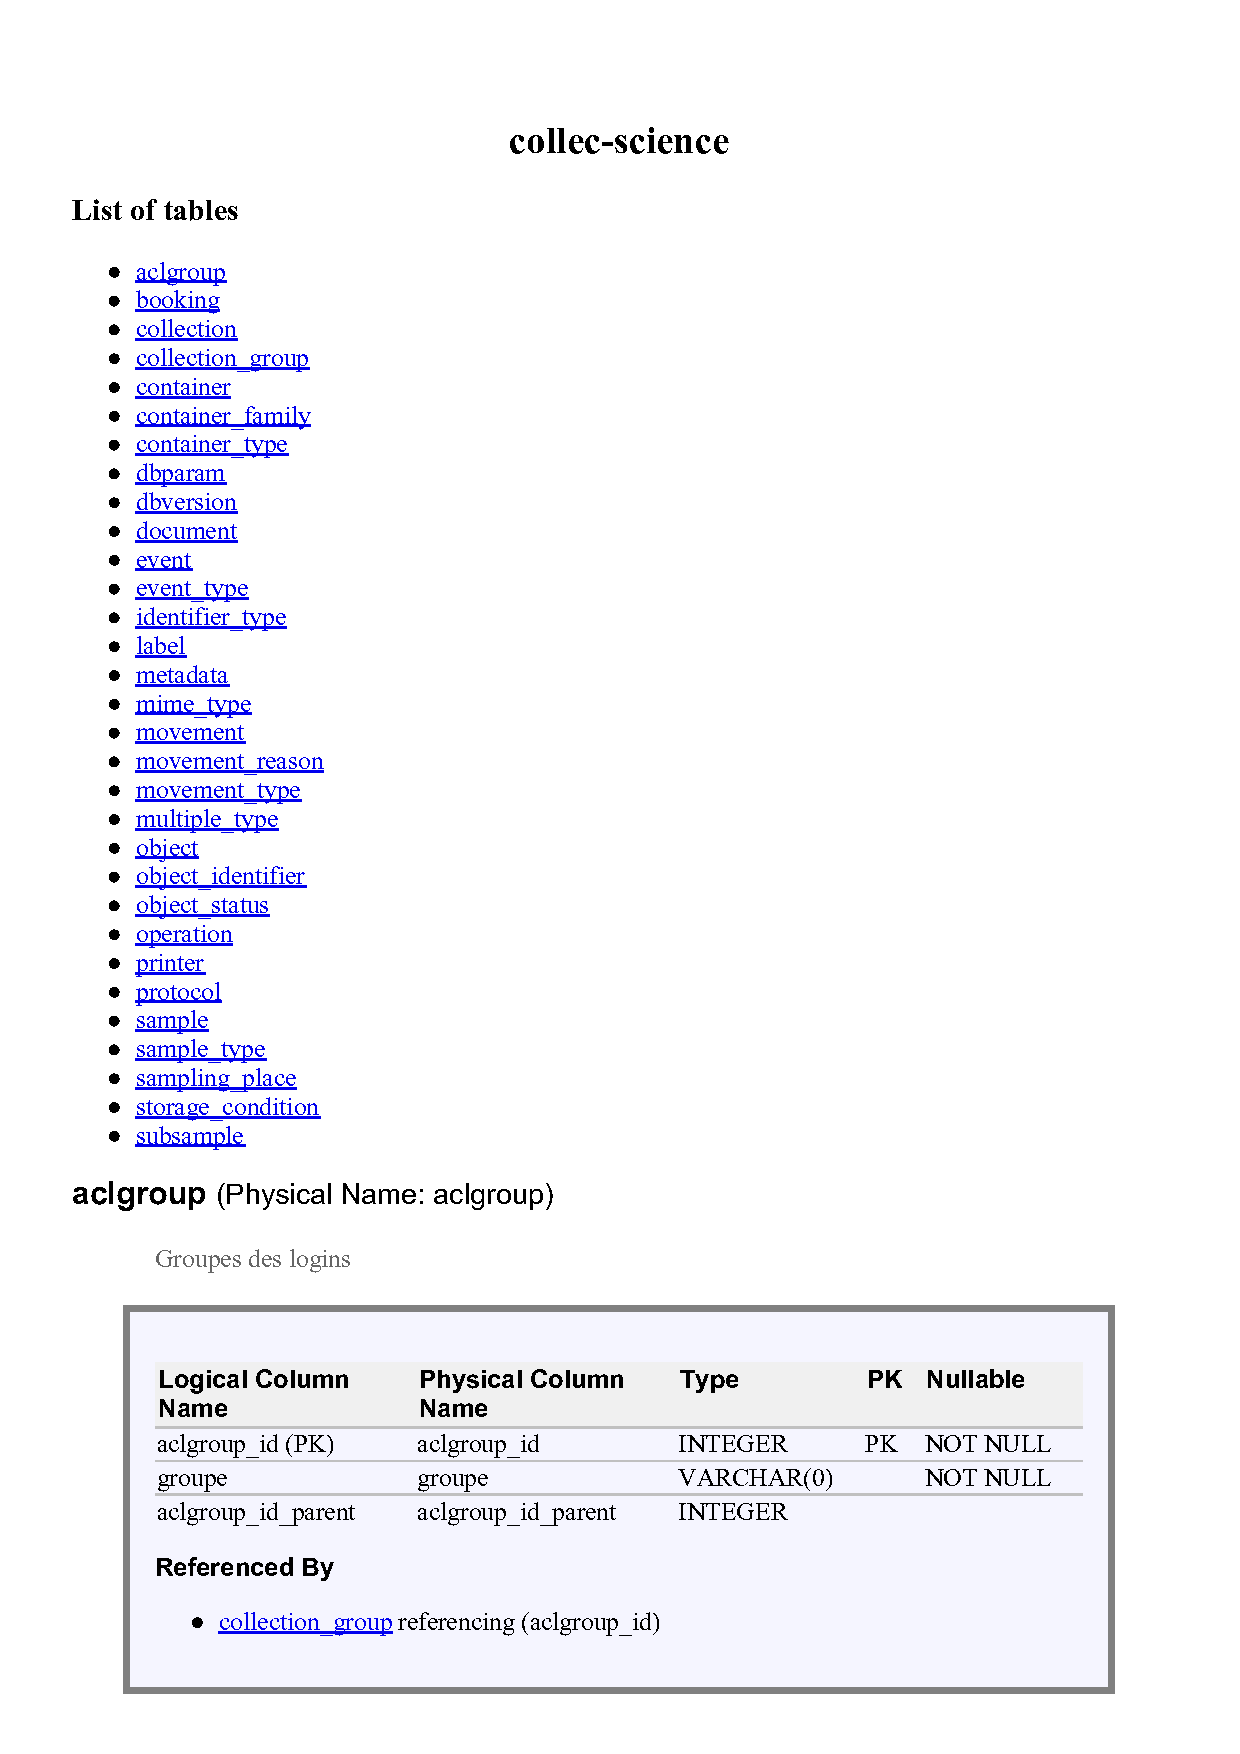
\includepdf[pages=1-17]{../collec-structure.pdf}

%Bibliographie
\backmatter

% Integration de la biblio
% Pour insérer toutes les références : 
%\nocite{*}
% Pour intégrer une référence non citée : 
%\nocite{ref}
\nocite{*}
\bibliography{collec}
\thispagestyle{empty}
\newgeometry{left=2cm,bottom=0.1cm}
\begin{center}
\color{inrae}
\vspace*{12cm}

\includegraphics[height=0.6cm]{fleche-titre}\par
\sffamily
EABX -- Écosystèmes aquatiques et changements globaux\\
50, avenue de Verdun\\
33612 CESTAS Cedex\\
+33 (0)5 57 89 08 00\par\bigskip
Rejoignez-nous sur :\\

\includegraphics{reseaux-sociaux}\par\bigskip
\vspace*{2cm}
{\bfseries Institut national de recherche pour\\
l'agriculture, l'alimentation et l'environnement}\par\bigskip
\vspace*{2cm}

\includegraphics[width=5cm]{blocmarque.jpg}




\end{center}
\restoregeometry
\end{document}